\documentclass[1p]{elsarticle_modified}
%\bibliographystyle{elsarticle-num}

%\usepackage[colorlinks]{hyperref}
%\usepackage{abbrmath_seonhwa} %\Abb, \Ascr, \Acal ,\Abf, \Afrak
\usepackage{amsfonts}
\usepackage{amssymb}
\usepackage{amsmath}
\usepackage{amsthm}
\usepackage{scalefnt}
\usepackage{amsbsy}
\usepackage{kotex}
\usepackage{caption}
\usepackage{subfig}
\usepackage{color}
\usepackage{graphicx}
\usepackage{xcolor} %% white, black, red, green, blue, cyan, magenta, yellow
\usepackage{float}
\usepackage{setspace}
\usepackage{hyperref}

\usepackage{tikz}
\usetikzlibrary{arrows}

\usepackage{multirow}
\usepackage{array} % fixed length table
\usepackage{hhline}

%%%%%%%%%%%%%%%%%%%%%
\makeatletter
\renewcommand*\env@matrix[1][\arraystretch]{%
	\edef\arraystretch{#1}%
	\hskip -\arraycolsep
	\let\@ifnextchar\new@ifnextchar
	\array{*\c@MaxMatrixCols c}}
\makeatother %https://tex.stackexchange.com/questions/14071/how-can-i-increase-the-line-spacing-in-a-matrix
%%%%%%%%%%%%%%%

\usepackage[normalem]{ulem}

\newcommand{\msout}[1]{\ifmmode\text{\sout{\ensuremath{#1}}}\else\sout{#1}\fi}
%SOURCE: \msout is \stkout macro in https://tex.stackexchange.com/questions/20609/strikeout-in-math-mode

\newcommand{\cancel}[1]{
	\ifmmode
	{\color{red}\msout{#1}}
	\else
	{\color{red}\sout{#1}}
	\fi
}

\newcommand{\add}[1]{
	{\color{blue}\uwave{#1}}
}

\newcommand{\replace}[2]{
	\ifmmode
	{\color{red}\msout{#1}}{\color{blue}\uwave{#2}}
	\else
	{\color{red}\sout{#1}}{\color{blue}\uwave{#2}}
	\fi
}

\newcommand{\Sol}{\mathcal{S}} %segment
\newcommand{\D}{D} %diagram
\newcommand{\A}{\mathcal{A}} %arc


%%%%%%%%%%%%%%%%%%%%%%%%%%%%%5 test

\def\sl{\operatorname{\textup{SL}}(2,\Cbb)}
\def\psl{\operatorname{\textup{PSL}}(2,\Cbb)}
\def\quan{\mkern 1mu \triangleright \mkern 1mu}

\theoremstyle{definition}
\newtheorem{thm}{Theorem}[section]
\newtheorem{prop}[thm]{Proposition}
\newtheorem{lem}[thm]{Lemma}
\newtheorem{ques}[thm]{Question}
\newtheorem{cor}[thm]{Corollary}
\newtheorem{defn}[thm]{Definition}
\newtheorem{exam}[thm]{Example}
\newtheorem{rmk}[thm]{Remark}
\newtheorem{alg}[thm]{Algorithm}

\newcommand{\I}{\sqrt{-1}}
\begin{document}

%\begin{frontmatter}
%
%\title{Boundary parabolic representations of knots up to 8 crossings}
%
%%% Group authors per affiliation:
%\author{Yunhi Cho} 
%\address{Department of Mathematics, University of Seoul, Seoul, Korea}
%\ead{yhcho@uos.ac.kr}
%
%
%\author{Seonhwa Kim} %\fnref{s_kim}}
%\address{Center for Geometry and Physics, Institute for Basic Science, Pohang, 37673, Korea}
%\ead{ryeona17@ibs.re.kr}
%
%\author{Hyuk Kim}
%\address{Department of Mathematical Sciences, Seoul National University, Seoul 08826, Korea}
%\ead{hyukkim@snu.ac.kr}
%
%\author{Seokbeom Yoon}
%\address{Department of Mathematical Sciences, Seoul National University, Seoul, 08826,  Korea}
%\ead{sbyoon15@snu.ac.kr}
%
%\begin{abstract}
%We find all boundary parabolic representation of knots up to 8 crossings.
%
%\end{abstract}
%\begin{keyword}
%    \MSC[2010] 57M25 
%\end{keyword}
%
%\end{frontmatter}

%\linenumbers
%\tableofcontents
%
\newcommand\colored[1]{\textcolor{white}{\rule[-0.35ex]{0.8em}{1.4ex}}\kern-0.8em\color{red} #1}%
%\newcommand\colored[1]{\textcolor{white}{ #1}\kern-2.17ex	\textcolor{white}{ #1}\kern-1.81ex	\textcolor{white}{ #1}\kern-2.15ex\color{red}#1	}

{\Large $\underline{12a_{0626}~(K12a_{0626})}$}

\setlength{\tabcolsep}{10pt}
\renewcommand{\arraystretch}{1.6}
\vspace{1cm}\begin{tabular}{m{100pt}>{\centering\arraybackslash}m{274pt}}
\multirow{5}{120pt}{
	\centering
	\includegraphics[width=112pt]{../../../GIT/diagram.site/Diagrams/png/1427_12a_0626.png}\\
\ \ \ A knot diagram\footnotemark}&
\allowdisplaybreaks
\textbf{Linearized knot diagam} \\
\cline{2-2}
 &
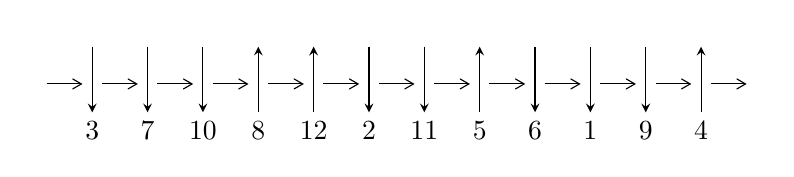
\begin{tikzpicture}[x=20pt, y=17pt]
	% nodes
	\node (C0) at (0, 0) {};
	\node (C1) at (1, 0) {};
	\node (C1U) at (1, +1) {};
	\node (C1D) at (1, -1) {3};

	\node (C2) at (2, 0) {};
	\node (C2U) at (2, +1) {};
	\node (C2D) at (2, -1) {7};

	\node (C3) at (3, 0) {};
	\node (C3U) at (3, +1) {};
	\node (C3D) at (3, -1) {10};

	\node (C4) at (4, 0) {};
	\node (C4U) at (4, +1) {};
	\node (C4D) at (4, -1) {8};

	\node (C5) at (5, 0) {};
	\node (C5U) at (5, +1) {};
	\node (C5D) at (5, -1) {12};

	\node (C6) at (6, 0) {};
	\node (C6U) at (6, +1) {};
	\node (C6D) at (6, -1) {2};

	\node (C7) at (7, 0) {};
	\node (C7U) at (7, +1) {};
	\node (C7D) at (7, -1) {11};

	\node (C8) at (8, 0) {};
	\node (C8U) at (8, +1) {};
	\node (C8D) at (8, -1) {5};

	\node (C9) at (9, 0) {};
	\node (C9U) at (9, +1) {};
	\node (C9D) at (9, -1) {6};

	\node (C10) at (10, 0) {};
	\node (C10U) at (10, +1) {};
	\node (C10D) at (10, -1) {1};

	\node (C11) at (11, 0) {};
	\node (C11U) at (11, +1) {};
	\node (C11D) at (11, -1) {9};

	\node (C12) at (12, 0) {};
	\node (C12U) at (12, +1) {};
	\node (C12D) at (12, -1) {4};
	\node (C13) at (13, 0) {};

	% arrows
	\draw[->,>={angle 60}]
	(C0) edge (C1) (C1) edge (C2) (C2) edge (C3) (C3) edge (C4) (C4) edge (C5) (C5) edge (C6) (C6) edge (C7) (C7) edge (C8) (C8) edge (C9) (C9) edge (C10) (C10) edge (C11) (C11) edge (C12) (C12) edge (C13) ;	\draw[->,>=stealth]
	(C1U) edge (C1D) (C2U) edge (C2D) (C3U) edge (C3D) (C4D) edge (C4U) (C5D) edge (C5U) (C6U) edge (C6D) (C7U) edge (C7D) (C8D) edge (C8U) (C9U) edge (C9D) (C10U) edge (C10D) (C11U) edge (C11D) (C12D) edge (C12U) ;
	\end{tikzpicture} \\
\hhline{~~} \\& 
\textbf{Solving Sequence} \\ \cline{2-2} 
 &
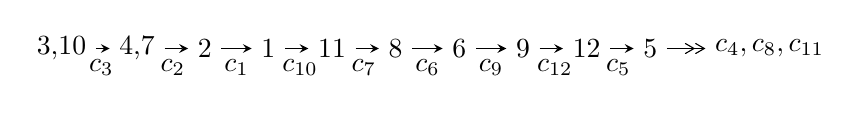
\begin{tikzpicture}[x=23pt, y=7pt]
	% node
	\node (A0) at (-1/8, 0) {3,10};
	\node (A1) at (17/16, 0) {4,7};
	\node (A2) at (17/8, 0) {2};
	\node (A3) at (25/8, 0) {1};
	\node (A4) at (33/8, 0) {11};
	\node (A5) at (41/8, 0) {8};
	\node (A6) at (49/8, 0) {6};
	\node (A7) at (57/8, 0) {9};
	\node (A8) at (65/8, 0) {12};
	\node (A9) at (73/8, 0) {5};
	\node (C1) at (1/2, -1) {$c_{3}$};
	\node (C2) at (13/8, -1) {$c_{2}$};
	\node (C3) at (21/8, -1) {$c_{1}$};
	\node (C4) at (29/8, -1) {$c_{10}$};
	\node (C5) at (37/8, -1) {$c_{7}$};
	\node (C6) at (45/8, -1) {$c_{6}$};
	\node (C7) at (53/8, -1) {$c_{9}$};
	\node (C8) at (61/8, -1) {$c_{12}$};
	\node (C9) at (69/8, -1) {$c_{5}$};
	\node (A10) at (11, 0) {$c_{4},c_{8},c_{11}$};

	% edge
	\draw[->,>=stealth]	
	(A0) edge (A1) (A1) edge (A2) (A2) edge (A3) (A3) edge (A4) (A4) edge (A5) (A5) edge (A6) (A6) edge (A7) (A7) edge (A8) (A8) edge (A9) ;
	\draw[->>,>={angle 60}]	
	(A9) edge (A10);
\end{tikzpicture} \\ 

\end{tabular} \\

\footnotetext{
The image of knot diagram is generated by the software ``\textbf{Draw programme}" developed by Andrew Bartholomew(\url{http://www.layer8.co.uk/maths/draw/index.htm\#Running-draw}), where we modified some parts for our purpose(\url{https://github.com/CATsTAILs/LinksPainter}).
}\phantom \\ \newline 
\centering \textbf{Ideals for irreducible components\footnotemark of $X_{\text{par}}$} 
 
\begin{align*}
I^u_{1}&=\langle 
7.86533\times10^{2128} u^{183}+1.64102\times10^{2128} u^{182}+\cdots+3.32893\times10^{2127} b-3.58156\times10^{2129},\\
\phantom{I^u_{1}}&\phantom{= \langle  }-4.72797\times10^{2128} u^{183}-2.22168\times10^{2128} u^{182}+\cdots+3.32893\times10^{2127} a+8.93000\times10^{2128},\\
\phantom{I^u_{1}}&\phantom{= \langle  }u^{184}-7 u^{182}+\cdots-48 u+1\rangle \\
I^u_{2}&=\langle 
2.34982\times10^{43} u^{36}+3.52408\times10^{43} u^{35}+\cdots+1.78735\times10^{44} b+4.37471\times10^{44},\\
\phantom{I^u_{2}}&\phantom{= \langle  }5.61215\times10^{42} u^{36}-9.92149\times10^{43} u^{35}+\cdots+1.78735\times10^{44} a-4.60729\times10^{44},\;u^{37}- u^{36}+\cdots+4 u-1\rangle \\
I^u_{3}&=\langle 
b-1,\;u^2+a- u,\;u^3- u^2+1\rangle \\
I^u_{4}&=\langle 
b-1,\;a,\;u+1\rangle \\
\\
\end{align*}
\raggedright * 4 irreducible components of $\dim_{\mathbb{C}}=0$, with total 225 representations.\\
\footnotetext{All coefficients of polynomials are rational numbers. But the coefficients are sometimes approximated in decimal forms when there is not enough margin.}
\newpage
\renewcommand{\arraystretch}{1}
\centering \section*{I. $I^u_{1}= \langle 7.87\times10^{2128} u^{183}+1.64\times10^{2128} u^{182}+\cdots+3.33\times10^{2127} b-3.58\times10^{2129},\;-4.73\times10^{2128} u^{183}-2.22\times10^{2128} u^{182}+\cdots+3.33\times10^{2127} a+8.93\times10^{2128},\;u^{184}-7 u^{182}+\cdots-48 u+1 \rangle$}
\flushleft \textbf{(i) Arc colorings}\\
\begin{tabular}{m{7pt} m{180pt} m{7pt} m{180pt} }
\flushright $a_{3}=$&$\begin{pmatrix}1\\0\end{pmatrix}$ \\
\flushright $a_{10}=$&$\begin{pmatrix}0\\u\end{pmatrix}$ \\
\flushright $a_{4}=$&$\begin{pmatrix}1\\u^2\end{pmatrix}$ \\
\flushright $a_{7}=$&$\begin{pmatrix}14.2027 u^{183}+6.67387 u^{182}+\cdots-351.805 u-26.8254\\-23.6272 u^{183}-4.92958 u^{182}+\cdots-4642.15 u+107.589\end{pmatrix}$ \\
\flushright $a_{2}=$&$\begin{pmatrix}143.075 u^{183}+20.7496 u^{182}+\cdots+37462.1 u-850.706\\45.1284 u^{183}+8.48457 u^{182}+\cdots+10158.6 u-236.205\end{pmatrix}$ \\
\flushright $a_{1}=$&$\begin{pmatrix}188.203 u^{183}+29.2342 u^{182}+\cdots+47620.7 u-1086.91\\45.1284 u^{183}+8.48457 u^{182}+\cdots+10158.6 u-236.205\end{pmatrix}$ \\
\flushright $a_{11}=$&$\begin{pmatrix}90.7028 u^{183}+29.7949 u^{182}+\cdots-4152.37 u+205.620\\44.6146 u^{183}+7.83308 u^{182}+\cdots+11173.8 u-266.852\end{pmatrix}$ \\
\flushright $a_{8}=$&$\begin{pmatrix}-23.7361 u^{183}-12.8653 u^{182}+\cdots+12346.1 u-382.439\\-37.5927 u^{183}-6.74894 u^{182}+\cdots-9175.95 u+218.649\end{pmatrix}$ \\
\flushright $a_{6}=$&$\begin{pmatrix}199.095 u^{183}+36.6781 u^{182}+\cdots+52161.6 u-1312.22\\21.0295 u^{183}+3.87033 u^{182}+\cdots+4688.83 u-107.085\end{pmatrix}$ \\
\flushright $a_{9}=$&$\begin{pmatrix}117.596 u^{183}+34.8904 u^{182}+\cdots-1564.59 u+215.030\\62.2326 u^{183}+11.7051 u^{182}+\cdots+14455.2 u-343.796\end{pmatrix}$ \\
\flushright $a_{12}=$&$\begin{pmatrix}147.569 u^{183}+21.4774 u^{182}+\cdots+38677.1 u-879.940\\43.6597 u^{183}+8.20677 u^{182}+\cdots+9826.91 u-228.448\end{pmatrix}$ \\
\flushright $a_{5}=$&$\begin{pmatrix}42.6808 u^{183}+13.3291 u^{182}+\cdots+3411.97 u-97.3779\\-1.28583 u^{183}-0.690805 u^{182}+\cdots+459.419 u-12.9308\end{pmatrix}$\\&\end{tabular}
\flushleft \textbf{(ii) Obstruction class $= -1$}\\~\\
\flushleft \textbf{(iii) Cusp Shapes $= -155.803 u^{183}-28.2047 u^{182}+\cdots-37929.8 u+907.606$}\\~\\
\newpage\renewcommand{\arraystretch}{1}
\flushleft \textbf{(iv) u-Polynomials at the component}\newline \\
\begin{tabular}{m{50pt}|m{274pt}}
Crossings & \hspace{64pt}u-Polynomials at each crossing \\
\hline $$\begin{aligned}c_{1}\end{aligned}$$&$\begin{aligned}
&u^{184}+79 u^{183}+\cdots+66 u+1
\end{aligned}$\\
\hline $$\begin{aligned}c_{2},c_{6}\end{aligned}$$&$\begin{aligned}
&u^{184}-3 u^{183}+\cdots-4 u-1
\end{aligned}$\\
\hline $$\begin{aligned}c_{3}\end{aligned}$$&$\begin{aligned}
&u^{184}-7 u^{182}+\cdots-48 u+1
\end{aligned}$\\
\hline $$\begin{aligned}c_{4},c_{8}\end{aligned}$$&$\begin{aligned}
&u^{184}-59 u^{182}+\cdots+22892 u+12427
\end{aligned}$\\
\hline $$\begin{aligned}c_{5}\end{aligned}$$&$\begin{aligned}
&u^{184}-3 u^{183}+\cdots-116 u+8
\end{aligned}$\\
\hline $$\begin{aligned}c_{7}\end{aligned}$$&$\begin{aligned}
&u^{184}-3 u^{183}+\cdots-12361749 u+6342353
\end{aligned}$\\
\hline $$\begin{aligned}c_{9}\end{aligned}$$&$\begin{aligned}
&u^{184}+5 u^{183}+\cdots+295470856 u-528012557
\end{aligned}$\\
\hline $$\begin{aligned}c_{10}\end{aligned}$$&$\begin{aligned}
&u^{184}+13 u^{183}+\cdots+40 u-1
\end{aligned}$\\
\hline $$\begin{aligned}c_{11}\end{aligned}$$&$\begin{aligned}
&u^{184}+15 u^{183}+\cdots-15 u+25
\end{aligned}$\\
\hline $$\begin{aligned}c_{12}\end{aligned}$$&$\begin{aligned}
&u^{184}+15 u^{183}+\cdots+30582126 u+2950777
\end{aligned}$\\
\hline
\end{tabular}\\~\\
\newpage\renewcommand{\arraystretch}{1}
\flushleft \textbf{(v) Riley Polynomials at the component}\newline \\
\begin{tabular}{m{50pt}|m{274pt}}
Crossings & \hspace{64pt}Riley Polynomials at each crossing \\
\hline $$\begin{aligned}c_{1}\end{aligned}$$&$\begin{aligned}
&y^{184}+61 y^{183}+\cdots+1678 y+1
\end{aligned}$\\
\hline $$\begin{aligned}c_{2},c_{6}\end{aligned}$$&$\begin{aligned}
&y^{184}-79 y^{183}+\cdots-66 y+1
\end{aligned}$\\
\hline $$\begin{aligned}c_{3}\end{aligned}$$&$\begin{aligned}
&y^{184}-14 y^{183}+\cdots-68 y+1
\end{aligned}$\\
\hline $$\begin{aligned}c_{4},c_{8}\end{aligned}$$&$\begin{aligned}
&y^{184}-118 y^{183}+\cdots-10917315406 y+154430329
\end{aligned}$\\
\hline $$\begin{aligned}c_{5}\end{aligned}$$&$\begin{aligned}
&y^{184}+y^{183}+\cdots-3536 y+64
\end{aligned}$\\
\hline $$\begin{aligned}c_{7}\end{aligned}$$&$\begin{aligned}
&y^{184}-45 y^{183}+\cdots-873004298058573 y+40225441576609
\end{aligned}$\\
\hline $$\begin{aligned}c_{9}\end{aligned}$$&$\begin{aligned}
&y^{184}-75 y^{183}+\cdots-1.97\times10^{19} y+2.79\times10^{17}
\end{aligned}$\\
\hline $$\begin{aligned}c_{10}\end{aligned}$$&$\begin{aligned}
&y^{184}+y^{183}+\cdots+34 y+1
\end{aligned}$\\
\hline $$\begin{aligned}c_{11}\end{aligned}$$&$\begin{aligned}
&y^{184}+7 y^{183}+\cdots-68925 y+625
\end{aligned}$\\
\hline $$\begin{aligned}c_{12}\end{aligned}$$&$\begin{aligned}
&y^{184}+69 y^{183}+\cdots+251263698396808 y+8707084903729
\end{aligned}$\\
\hline
\end{tabular}\\~\\
\newpage\flushleft \textbf{(vi) Complex Volumes and Cusp Shapes}
$$\begin{array}{c|c|c}  
\text{Solutions to }I^u_{1}& \I (\text{vol} + \sqrt{-1}CS) & \text{Cusp shape}\\
 \hline 
\begin{aligned}
u &= -0.988796 + 0.151009 I \\
a &= -0.123078 - 0.275216 I \\
b &= \phantom{-}1.086630 + 0.123254 I\end{aligned}
 & -1.64795 + 0.01014 I & \phantom{-0.000000 } 0 \\ \hline\begin{aligned}
u &= -0.988796 - 0.151009 I \\
a &= -0.123078 + 0.275216 I \\
b &= \phantom{-}1.086630 - 0.123254 I\end{aligned}
 & -1.64795 - 0.01014 I & \phantom{-0.000000 } 0 \\ \hline\begin{aligned}
u &= \phantom{-}0.148896 + 0.988387 I \\
a &= \phantom{-}0.20037 + 2.37336 I \\
b &= -0.805346 - 0.421075 I\end{aligned}
 & -1.96495 - 1.26789 I & \phantom{-0.000000 } 0 \\ \hline\begin{aligned}
u &= \phantom{-}0.148896 - 0.988387 I \\
a &= \phantom{-}0.20037 - 2.37336 I \\
b &= -0.805346 + 0.421075 I\end{aligned}
 & -1.96495 + 1.26789 I & \phantom{-0.000000 } 0 \\ \hline\begin{aligned}
u &= -0.993627 + 0.177595 I \\
a &= \phantom{-}0.490822 + 0.089141 I \\
b &= \phantom{-}0.657938 + 0.218229 I\end{aligned}
 & -1.48461 + 0.05604 I & \phantom{-0.000000 } 0 \\ \hline\begin{aligned}
u &= -0.993627 - 0.177595 I \\
a &= \phantom{-}0.490822 - 0.089141 I \\
b &= \phantom{-}0.657938 - 0.218229 I\end{aligned}
 & -1.48461 - 0.05604 I & \phantom{-0.000000 } 0 \\ \hline\begin{aligned}
u &= -0.767288 + 0.673975 I \\
a &= -0.817072 - 0.214175 I \\
b &= \phantom{-}0.268200 - 0.069839 I\end{aligned}
 & -0.92285 + 3.03118 I & \phantom{-0.000000 } 0 \\ \hline\begin{aligned}
u &= -0.767288 - 0.673975 I \\
a &= -0.817072 + 0.214175 I \\
b &= \phantom{-}0.268200 + 0.069839 I\end{aligned}
 & -0.92285 - 3.03118 I & \phantom{-0.000000 } 0 \\ \hline\begin{aligned}
u &= \phantom{-}0.644715 + 0.723596 I \\
a &= -0.20569 + 1.56336 I \\
b &= -1.165230 - 0.656934 I\end{aligned}
 & -1.50318 - 8.74117 I & \phantom{-0.000000 } 0 \\ \hline\begin{aligned}
u &= \phantom{-}0.644715 - 0.723596 I \\
a &= -0.20569 - 1.56336 I \\
b &= -1.165230 + 0.656934 I\end{aligned}
 & -1.50318 + 8.74117 I & \phantom{-0.000000 } 0\\
 \hline 
 \end{array}$$\newpage$$\begin{array}{c|c|c}  
\text{Solutions to }I^u_{1}& \I (\text{vol} + \sqrt{-1}CS) & \text{Cusp shape}\\
 \hline 
\begin{aligned}
u &= -0.979304 + 0.332875 I \\
a &= \phantom{-}0.737503 + 0.966815 I \\
b &= \phantom{-}0.988373 + 0.350195 I\end{aligned}
 & -1.79371 + 5.24195 I & \phantom{-0.000000 } 0 \\ \hline\begin{aligned}
u &= -0.979304 - 0.332875 I \\
a &= \phantom{-}0.737503 - 0.966815 I \\
b &= \phantom{-}0.988373 - 0.350195 I\end{aligned}
 & -1.79371 - 5.24195 I & \phantom{-0.000000 } 0 \\ \hline\begin{aligned}
u &= \phantom{-}0.928414 + 0.200321 I \\
a &= -1.59659 - 0.19661 I \\
b &= -0.947327 - 0.369105 I\end{aligned}
 & -3.80906 - 3.52196 I & \phantom{-0.000000 } 0 \\ \hline\begin{aligned}
u &= \phantom{-}0.928414 - 0.200321 I \\
a &= -1.59659 + 0.19661 I \\
b &= -0.947327 + 0.369105 I\end{aligned}
 & -3.80906 + 3.52196 I & \phantom{-0.000000 } 0 \\ \hline\begin{aligned}
u &= -0.809600 + 0.680889 I \\
a &= \phantom{-}0.384132 + 0.730998 I \\
b &= -0.418408 - 0.936783 I\end{aligned}
 & \phantom{-}0.32628 + 3.28163 I & \phantom{-0.000000 } 0 \\ \hline\begin{aligned}
u &= -0.809600 - 0.680889 I \\
a &= \phantom{-}0.384132 - 0.730998 I \\
b &= -0.418408 + 0.936783 I\end{aligned}
 & \phantom{-}0.32628 - 3.28163 I & \phantom{-0.000000 } 0 \\ \hline\begin{aligned}
u &= \phantom{-}0.605967 + 0.870951 I \\
a &= -0.018067 - 1.244780 I \\
b &= \phantom{-}0.116387 + 0.868823 I\end{aligned}
 & \phantom{-}2.64975 - 4.01921 I & \phantom{-0.000000 } 0 \\ \hline\begin{aligned}
u &= \phantom{-}0.605967 - 0.870951 I \\
a &= -0.018067 + 1.244780 I \\
b &= \phantom{-}0.116387 - 0.868823 I\end{aligned}
 & \phantom{-}2.64975 + 4.01921 I & \phantom{-0.000000 } 0 \\ \hline\begin{aligned}
u &= \phantom{-}0.366462 + 0.843695 I \\
a &= \phantom{-}0.653044 - 1.222880 I \\
b &= -0.596664 + 0.701241 I\end{aligned}
 & \phantom{-}2.84886 + 0.00272 I & \phantom{-0.000000 } 0 \\ \hline\begin{aligned}
u &= \phantom{-}0.366462 - 0.843695 I \\
a &= \phantom{-}0.653044 + 1.222880 I \\
b &= -0.596664 - 0.701241 I\end{aligned}
 & \phantom{-}2.84886 - 0.00272 I & \phantom{-0.000000 } 0\\
 \hline 
 \end{array}$$\newpage$$\begin{array}{c|c|c}  
\text{Solutions to }I^u_{1}& \I (\text{vol} + \sqrt{-1}CS) & \text{Cusp shape}\\
 \hline 
\begin{aligned}
u &= -0.699561 + 0.827120 I \\
a &= \phantom{-}0.91193 + 2.11073 I \\
b &= \phantom{-}1.005720 - 0.639870 I\end{aligned}
 & \phantom{-}3.87100 + 11.85910 I & \phantom{-0.000000 } 0 \\ \hline\begin{aligned}
u &= -0.699561 - 0.827120 I \\
a &= \phantom{-}0.91193 - 2.11073 I \\
b &= \phantom{-}1.005720 + 0.639870 I\end{aligned}
 & \phantom{-}3.87100 - 11.85910 I & \phantom{-0.000000 } 0 \\ \hline\begin{aligned}
u &= \phantom{-}1.052930 + 0.255822 I \\
a &= -0.654819 - 0.313006 I \\
b &= -1.198340 - 0.031092 I\end{aligned}
 & -5.54921 - 3.55445 I & \phantom{-0.000000 } 0 \\ \hline\begin{aligned}
u &= \phantom{-}1.052930 - 0.255822 I \\
a &= -0.654819 + 0.313006 I \\
b &= -1.198340 + 0.031092 I\end{aligned}
 & -5.54921 + 3.55445 I & \phantom{-0.000000 } 0 \\ \hline\begin{aligned}
u &= \phantom{-}0.888043 + 0.217629 I \\
a &= \phantom{-}1.220600 + 0.097137 I \\
b &= \phantom{-}1.082100 + 0.417541 I\end{aligned}
 & -2.32112 - 6.87988 I & \phantom{-0.000000 } 0 \\ \hline\begin{aligned}
u &= \phantom{-}0.888043 - 0.217629 I \\
a &= \phantom{-}1.220600 - 0.097137 I \\
b &= \phantom{-}1.082100 - 0.417541 I\end{aligned}
 & -2.32112 + 6.87988 I & \phantom{-0.000000 } 0 \\ \hline\begin{aligned}
u &= \phantom{-}0.546999 + 0.940381 I \\
a &= \phantom{-}0.903420 - 0.953240 I \\
b &= -0.595553 + 0.756202 I\end{aligned}
 & \phantom{-}2.90265 - 0.21493 I & \phantom{-0.000000 } 0 \\ \hline\begin{aligned}
u &= \phantom{-}0.546999 - 0.940381 I \\
a &= \phantom{-}0.903420 + 0.953240 I \\
b &= -0.595553 - 0.756202 I\end{aligned}
 & \phantom{-}2.90265 + 0.21493 I & \phantom{-0.000000 } 0 \\ \hline\begin{aligned}
u &= \phantom{-}0.817498 + 0.731479 I \\
a &= -0.265860 + 1.341890 I \\
b &= \phantom{-}0.081161 - 0.318220 I\end{aligned}
 & -2.73921 + 2.06070 I & \phantom{-0.000000 } 0 \\ \hline\begin{aligned}
u &= \phantom{-}0.817498 - 0.731479 I \\
a &= -0.265860 - 1.341890 I \\
b &= \phantom{-}0.081161 + 0.318220 I\end{aligned}
 & -2.73921 - 2.06070 I & \phantom{-0.000000 } 0\\
 \hline 
 \end{array}$$\newpage$$\begin{array}{c|c|c}  
\text{Solutions to }I^u_{1}& \I (\text{vol} + \sqrt{-1}CS) & \text{Cusp shape}\\
 \hline 
\begin{aligned}
u &= -0.800089 + 0.417080 I \\
a &= -0.02237 - 1.55738 I \\
b &= -0.922984 - 0.399840 I\end{aligned}
 & -3.86517 + 0.54090 I & \phantom{-0.000000 } 0 \\ \hline\begin{aligned}
u &= -0.800089 - 0.417080 I \\
a &= -0.02237 + 1.55738 I \\
b &= -0.922984 + 0.399840 I\end{aligned}
 & -3.86517 - 0.54090 I & \phantom{-0.000000 } 0 \\ \hline\begin{aligned}
u &= \phantom{-}0.884671 + 0.165116 I \\
a &= \phantom{-}0.428900 + 0.168466 I \\
b &= \phantom{-}1.306710 - 0.028320 I\end{aligned}
 & -6.09985 - 0.31423 I & \phantom{-0.000000 } 0 \\ \hline\begin{aligned}
u &= \phantom{-}0.884671 - 0.165116 I \\
a &= \phantom{-}0.428900 - 0.168466 I \\
b &= \phantom{-}1.306710 + 0.028320 I\end{aligned}
 & -6.09985 + 0.31423 I & \phantom{-0.000000 } 0 \\ \hline\begin{aligned}
u &= \phantom{-}0.791100 + 0.396311 I \\
a &= \phantom{-}0.76895 - 1.31796 I \\
b &= -0.116475 - 0.128008 I\end{aligned}
 & \phantom{-}0.59351 + 7.58137 I & \phantom{-0.000000 } 0 \\ \hline\begin{aligned}
u &= \phantom{-}0.791100 - 0.396311 I \\
a &= \phantom{-}0.76895 + 1.31796 I \\
b &= -0.116475 + 0.128008 I\end{aligned}
 & \phantom{-}0.59351 - 7.58137 I & \phantom{-0.000000 } 0 \\ \hline\begin{aligned}
u &= -0.225789 + 0.832772 I \\
a &= -0.28666 - 1.58106 I \\
b &= -0.751134 + 0.629681 I\end{aligned}
 & \phantom{-}3.31513 + 0.13206 I & \phantom{-0.000000 } 0 \\ \hline\begin{aligned}
u &= -0.225789 - 0.832772 I \\
a &= -0.28666 + 1.58106 I \\
b &= -0.751134 - 0.629681 I\end{aligned}
 & \phantom{-}3.31513 - 0.13206 I & \phantom{-0.000000 } 0 \\ \hline\begin{aligned}
u &= \phantom{-}0.610002 + 0.961286 I \\
a &= -1.125400 + 0.512298 I \\
b &= \phantom{-}0.624395 - 0.740317 I\end{aligned}
 & \phantom{-}5.02536 - 6.59589 I & \phantom{-0.000000 } 0 \\ \hline\begin{aligned}
u &= \phantom{-}0.610002 - 0.961286 I \\
a &= -1.125400 - 0.512298 I \\
b &= \phantom{-}0.624395 + 0.740317 I\end{aligned}
 & \phantom{-}5.02536 + 6.59589 I & \phantom{-0.000000 } 0\\
 \hline 
 \end{array}$$\newpage$$\begin{array}{c|c|c}  
\text{Solutions to }I^u_{1}& \I (\text{vol} + \sqrt{-1}CS) & \text{Cusp shape}\\
 \hline 
\begin{aligned}
u &= -0.836010 + 0.206117 I \\
a &= \phantom{-}0.688519 + 0.174392 I \\
b &= \phantom{-}0.282847 + 0.028212 I\end{aligned}
 & -1.46001 + 0.11234 I & \phantom{-0.000000 } 0 \\ \hline\begin{aligned}
u &= -0.836010 - 0.206117 I \\
a &= \phantom{-}0.688519 - 0.174392 I \\
b &= \phantom{-}0.282847 - 0.028212 I\end{aligned}
 & -1.46001 - 0.11234 I & \phantom{-0.000000 } 0 \\ \hline\begin{aligned}
u &= -0.206240 + 1.135670 I \\
a &= -0.271797 - 0.934312 I \\
b &= \phantom{-}0.304957 + 0.915768 I\end{aligned}
 & \phantom{-}5.90118 + 6.01032 I & \phantom{-0.000000 } 0 \\ \hline\begin{aligned}
u &= -0.206240 - 1.135670 I \\
a &= -0.271797 + 0.934312 I \\
b &= \phantom{-}0.304957 - 0.915768 I\end{aligned}
 & \phantom{-}5.90118 - 6.01032 I & \phantom{-0.000000 } 0 \\ \hline\begin{aligned}
u &= \phantom{-}0.819430 + 0.164630 I \\
a &= \phantom{-}0.024107 - 1.186860 I \\
b &= -0.562324 + 0.794669 I\end{aligned}
 & \phantom{-}2.35368 - 2.23949 I & \phantom{-0.000000 } 0 \\ \hline\begin{aligned}
u &= \phantom{-}0.819430 - 0.164630 I \\
a &= \phantom{-}0.024107 + 1.186860 I \\
b &= -0.562324 - 0.794669 I\end{aligned}
 & \phantom{-}2.35368 + 2.23949 I & \phantom{-0.000000 } 0 \\ \hline\begin{aligned}
u &= -0.644932 + 0.971777 I \\
a &= \phantom{-}0.06540 - 1.66131 I \\
b &= -1.013040 + 0.616866 I\end{aligned}
 & \phantom{-}1.59880 + 5.08361 I & \phantom{-0.000000 } 0 \\ \hline\begin{aligned}
u &= -0.644932 - 0.971777 I \\
a &= \phantom{-}0.06540 + 1.66131 I \\
b &= -1.013040 - 0.616866 I\end{aligned}
 & \phantom{-}1.59880 - 5.08361 I & \phantom{-0.000000 } 0 \\ \hline\begin{aligned}
u &= -0.680805 + 0.951612 I \\
a &= -0.28340 - 1.99588 I \\
b &= -1.017460 + 0.646352 I\end{aligned}
 & \phantom{-}1.63829 + 5.53928 I & \phantom{-0.000000 } 0 \\ \hline\begin{aligned}
u &= -0.680805 - 0.951612 I \\
a &= -0.28340 + 1.99588 I \\
b &= -1.017460 - 0.646352 I\end{aligned}
 & \phantom{-}1.63829 - 5.53928 I & \phantom{-0.000000 } 0\\
 \hline 
 \end{array}$$\newpage$$\begin{array}{c|c|c}  
\text{Solutions to }I^u_{1}& \I (\text{vol} + \sqrt{-1}CS) & \text{Cusp shape}\\
 \hline 
\begin{aligned}
u &= \phantom{-}1.146400 + 0.238171 I \\
a &= \phantom{-}0.679781 + 0.079006 I \\
b &= \phantom{-}0.997314 - 0.489322 I\end{aligned}
 & -2.81614 + 3.74126 I & \phantom{-0.000000 } 0 \\ \hline\begin{aligned}
u &= \phantom{-}1.146400 - 0.238171 I \\
a &= \phantom{-}0.679781 - 0.079006 I \\
b &= \phantom{-}0.997314 + 0.489322 I\end{aligned}
 & -2.81614 - 3.74126 I & \phantom{-0.000000 } 0 \\ \hline\begin{aligned}
u &= -0.237276 + 1.160650 I \\
a &= \phantom{-}0.617156 - 0.614446 I \\
b &= -0.683102 + 0.461759 I\end{aligned}
 & \phantom{-}2.89008 + 4.52282 I & \phantom{-0.000000 } 0 \\ \hline\begin{aligned}
u &= -0.237276 - 1.160650 I \\
a &= \phantom{-}0.617156 + 0.614446 I \\
b &= -0.683102 - 0.461759 I\end{aligned}
 & \phantom{-}2.89008 - 4.52282 I & \phantom{-0.000000 } 0 \\ \hline\begin{aligned}
u &= \phantom{-}0.239699 + 1.181420 I \\
a &= -0.086171 + 1.174800 I \\
b &= \phantom{-}0.658187 - 0.787100 I\end{aligned}
 & \phantom{-}3.51167 + 0.15515 I & \phantom{-0.000000 } 0 \\ \hline\begin{aligned}
u &= \phantom{-}0.239699 - 1.181420 I \\
a &= -0.086171 - 1.174800 I \\
b &= \phantom{-}0.658187 + 0.787100 I\end{aligned}
 & \phantom{-}3.51167 - 0.15515 I & \phantom{-0.000000 } 0 \\ \hline\begin{aligned}
u &= \phantom{-}0.621187 + 0.486178 I \\
a &= -0.24085 + 2.92636 I \\
b &= -0.972251 - 0.391998 I\end{aligned}
 & -3.48361 - 2.08740 I & \phantom{-0.000000 } 0 \\ \hline\begin{aligned}
u &= \phantom{-}0.621187 - 0.486178 I \\
a &= -0.24085 - 2.92636 I \\
b &= -0.972251 + 0.391998 I\end{aligned}
 & -3.48361 + 2.08740 I & \phantom{-0.000000 } 0 \\ \hline\begin{aligned}
u &= -0.010233 + 1.218620 I \\
a &= \phantom{-}0.637640 - 0.769827 I \\
b &= -0.853997 + 0.571053 I\end{aligned}
 & \phantom{-}3.03021 + 4.63784 I & \phantom{-0.000000 } 0 \\ \hline\begin{aligned}
u &= -0.010233 - 1.218620 I \\
a &= \phantom{-}0.637640 + 0.769827 I \\
b &= -0.853997 - 0.571053 I\end{aligned}
 & \phantom{-}3.03021 - 4.63784 I & \phantom{-0.000000 } 0\\
 \hline 
 \end{array}$$\newpage$$\begin{array}{c|c|c}  
\text{Solutions to }I^u_{1}& \I (\text{vol} + \sqrt{-1}CS) & \text{Cusp shape}\\
 \hline 
\begin{aligned}
u &= \phantom{-}0.915152 + 0.806829 I \\
a &= \phantom{-}0.396078 + 0.567429 I \\
b &= \phantom{-}1.228310 - 0.243811 I\end{aligned}
 & -3.89959 - 3.03826 I & \phantom{-0.000000 } 0 \\ \hline\begin{aligned}
u &= \phantom{-}0.915152 - 0.806829 I \\
a &= \phantom{-}0.396078 - 0.567429 I \\
b &= \phantom{-}1.228310 + 0.243811 I\end{aligned}
 & -3.89959 + 3.03826 I & \phantom{-0.000000 } 0 \\ \hline\begin{aligned}
u &= -0.738444 + 0.986074 I \\
a &= \phantom{-}0.52162 + 1.53264 I \\
b &= \phantom{-}0.992293 - 0.651252 I\end{aligned}
 & \phantom{-}7.00532 + 2.40995 I & \phantom{-0.000000 } 0 \\ \hline\begin{aligned}
u &= -0.738444 - 0.986074 I \\
a &= \phantom{-}0.52162 - 1.53264 I \\
b &= \phantom{-}0.992293 + 0.651252 I\end{aligned}
 & \phantom{-}7.00532 - 2.40995 I & \phantom{-0.000000 } 0 \\ \hline\begin{aligned}
u &= \phantom{-}0.490626 + 1.137570 I \\
a &= -0.638821 + 0.671041 I \\
b &= \phantom{-}0.639745 - 0.749087 I\end{aligned}
 & \phantom{-}8.06893 + 2.90952 I & \phantom{-0.000000 } 0 \\ \hline\begin{aligned}
u &= \phantom{-}0.490626 - 1.137570 I \\
a &= -0.638821 - 0.671041 I \\
b &= \phantom{-}0.639745 + 0.749087 I\end{aligned}
 & \phantom{-}8.06893 - 2.90952 I & \phantom{-0.000000 } 0 \\ \hline\begin{aligned}
u &= -0.608705 + 0.456085 I \\
a &= \phantom{-}0.012049 + 1.135360 I \\
b &= \phantom{-}1.213310 - 0.620356 I\end{aligned}
 & -3.48102 + 2.76325 I & \phantom{-0.000000 } 0 \\ \hline\begin{aligned}
u &= -0.608705 - 0.456085 I \\
a &= \phantom{-}0.012049 - 1.135360 I \\
b &= \phantom{-}1.213310 + 0.620356 I\end{aligned}
 & -3.48102 - 2.76325 I & \phantom{-0.000000 } 0 \\ \hline\begin{aligned}
u &= -0.120210 + 0.742461 I \\
a &= -0.067714 - 0.947759 I \\
b &= -1.289460 + 0.424798 I\end{aligned}
 & \phantom{-}0.95584 - 1.90857 I & \phantom{-0.000000 } 0 \\ \hline\begin{aligned}
u &= -0.120210 - 0.742461 I \\
a &= -0.067714 + 0.947759 I \\
b &= -1.289460 - 0.424798 I\end{aligned}
 & \phantom{-}0.95584 + 1.90857 I & \phantom{-0.000000 } 0\\
 \hline 
 \end{array}$$\newpage$$\begin{array}{c|c|c}  
\text{Solutions to }I^u_{1}& \I (\text{vol} + \sqrt{-1}CS) & \text{Cusp shape}\\
 \hline 
\begin{aligned}
u &= -1.072180 + 0.651798 I \\
a &= \phantom{-}0.241556 - 0.100444 I \\
b &= \phantom{-}1.303820 + 0.028731 I\end{aligned}
 & -4.34400 + 12.61830 I & \phantom{-0.000000 } 0 \\ \hline\begin{aligned}
u &= -1.072180 - 0.651798 I \\
a &= \phantom{-}0.241556 + 0.100444 I \\
b &= \phantom{-}1.303820 - 0.028731 I\end{aligned}
 & -4.34400 - 12.61830 I & \phantom{-0.000000 } 0 \\ \hline\begin{aligned}
u &= -0.535290 + 0.515973 I \\
a &= \phantom{-}0.186309 + 0.165691 I \\
b &= \phantom{-}0.096573 + 0.756436 I\end{aligned}
 & \phantom{-}0.70702 + 2.88973 I & \phantom{-0.000000 } 0 \\ \hline\begin{aligned}
u &= -0.535290 - 0.515973 I \\
a &= \phantom{-}0.186309 - 0.165691 I \\
b &= \phantom{-}0.096573 - 0.756436 I\end{aligned}
 & \phantom{-}0.70702 - 2.88973 I & \phantom{-0.000000 } 0 \\ \hline\begin{aligned}
u &= -1.25758\phantom{ +0.000000I} \\
a &= -0.239948\phantom{ +0.000000I} \\
b &= \phantom{-}1.34959\phantom{ +0.000000I}\end{aligned}
 & -2.30073\phantom{ +0.000000I} & \phantom{-0.000000 } 0 \\ \hline\begin{aligned}
u &= -1.119740 + 0.604025 I \\
a &= -0.183593 + 0.024877 I \\
b &= -1.287730 - 0.022879 I\end{aligned}
 & -8.21160 + 6.57180 I & \phantom{-0.000000 } 0 \\ \hline\begin{aligned}
u &= -1.119740 - 0.604025 I \\
a &= -0.183593 - 0.024877 I \\
b &= -1.287730 + 0.022879 I\end{aligned}
 & -8.21160 - 6.57180 I & \phantom{-0.000000 } 0 \\ \hline\begin{aligned}
u &= \phantom{-}0.497512 + 1.177230 I \\
a &= \phantom{-}0.093685 - 1.291900 I \\
b &= \phantom{-}1.192750 + 0.628651 I\end{aligned}
 & \phantom{-}3.24511 - 11.66680 I & \phantom{-0.000000 } 0 \\ \hline\begin{aligned}
u &= \phantom{-}0.497512 - 1.177230 I \\
a &= \phantom{-}0.093685 + 1.291900 I \\
b &= \phantom{-}1.192750 - 0.628651 I\end{aligned}
 & \phantom{-}3.24511 + 11.66680 I & \phantom{-0.000000 } 0 \\ \hline\begin{aligned}
u &= \phantom{-}1.025210 + 0.773394 I \\
a &= -0.354355 + 1.364630 I \\
b &= -1.150710 - 0.654347 I\end{aligned}
 & -1.91027 - 9.07572 I & \phantom{-0.000000 } 0\\
 \hline 
 \end{array}$$\newpage$$\begin{array}{c|c|c}  
\text{Solutions to }I^u_{1}& \I (\text{vol} + \sqrt{-1}CS) & \text{Cusp shape}\\
 \hline 
\begin{aligned}
u &= \phantom{-}1.025210 - 0.773394 I \\
a &= -0.354355 - 1.364630 I \\
b &= -1.150710 + 0.654347 I\end{aligned}
 & -1.91027 + 9.07572 I & \phantom{-0.000000 } 0 \\ \hline\begin{aligned}
u &= \phantom{-}0.683652 + 0.123417 I \\
a &= \phantom{-}1.03402 - 2.90910 I \\
b &= \phantom{-}0.956229 + 0.371239 I\end{aligned}
 & -2.58461 + 0.57570 I & \phantom{-0.000000 } 0 \\ \hline\begin{aligned}
u &= \phantom{-}0.683652 - 0.123417 I \\
a &= \phantom{-}1.03402 + 2.90910 I \\
b &= \phantom{-}0.956229 - 0.371239 I\end{aligned}
 & -2.58461 - 0.57570 I & \phantom{-0.000000 } 0 \\ \hline\begin{aligned}
u &= -1.254780 + 0.403077 I \\
a &= -0.003847 - 1.115490 I \\
b &= -1.089030 + 0.666055 I\end{aligned}
 & \phantom{-}0.73727 + 7.82190 I & \phantom{-0.000000 } 0 \\ \hline\begin{aligned}
u &= -1.254780 - 0.403077 I \\
a &= -0.003847 + 1.115490 I \\
b &= -1.089030 - 0.666055 I\end{aligned}
 & \phantom{-}0.73727 - 7.82190 I & \phantom{-0.000000 } 0 \\ \hline\begin{aligned}
u &= -0.539808 + 0.399048 I \\
a &= -0.379461 - 0.019512 I \\
b &= \phantom{-}0.178352 - 0.753086 I\end{aligned}
 & -0.417406 + 1.227370 I & \phantom{-0.000000 } 0 \\ \hline\begin{aligned}
u &= -0.539808 - 0.399048 I \\
a &= -0.379461 + 0.019512 I \\
b &= \phantom{-}0.178352 + 0.753086 I\end{aligned}
 & -0.417406 - 1.227370 I & \phantom{-0.000000 } 0 \\ \hline\begin{aligned}
u &= \phantom{-}0.342939 + 0.556689 I \\
a &= \phantom{-}0.687706 + 0.922412 I \\
b &= -0.648194 - 1.004410 I\end{aligned}
 & \phantom{-}3.17591 - 10.18350 I & \phantom{-0.000000 } 0 \\ \hline\begin{aligned}
u &= \phantom{-}0.342939 - 0.556689 I \\
a &= \phantom{-}0.687706 - 0.922412 I \\
b &= -0.648194 + 1.004410 I\end{aligned}
 & \phantom{-}3.17591 + 10.18350 I & \phantom{-0.000000 } 0 \\ \hline\begin{aligned}
u &= -1.108430 + 0.773328 I \\
a &= -0.273605 - 0.738251 I \\
b &= \phantom{-}0.521586 + 0.922379 I\end{aligned}
 & \phantom{-}1.09909 + 5.49407 I & \phantom{-0.000000 } 0\\
 \hline 
 \end{array}$$\newpage$$\begin{array}{c|c|c}  
\text{Solutions to }I^u_{1}& \I (\text{vol} + \sqrt{-1}CS) & \text{Cusp shape}\\
 \hline 
\begin{aligned}
u &= -1.108430 - 0.773328 I \\
a &= -0.273605 + 0.738251 I \\
b &= \phantom{-}0.521586 - 0.922379 I\end{aligned}
 & \phantom{-}1.09909 - 5.49407 I & \phantom{-0.000000 } 0 \\ \hline\begin{aligned}
u &= -0.281449 + 0.559280 I \\
a &= \phantom{-}0.585901 + 0.960879 I \\
b &= -0.353996 - 0.980175 I\end{aligned}
 & \phantom{-}0.91017 + 2.86934 I & \phantom{-0.000000 } 0 \\ \hline\begin{aligned}
u &= -0.281449 - 0.559280 I \\
a &= \phantom{-}0.585901 - 0.960879 I \\
b &= -0.353996 + 0.980175 I\end{aligned}
 & \phantom{-}0.91017 - 2.86934 I & \phantom{-0.000000 } 0 \\ \hline\begin{aligned}
u &= -0.260479 + 0.568461 I \\
a &= -0.311477 + 0.124225 I \\
b &= \phantom{-}0.425433 - 0.588214 I\end{aligned}
 & -0.37471 + 1.71454 I & \phantom{-0.000000 } 0 \\ \hline\begin{aligned}
u &= -0.260479 - 0.568461 I \\
a &= -0.311477 - 0.124225 I \\
b &= \phantom{-}0.425433 + 0.588214 I\end{aligned}
 & -0.37471 - 1.71454 I & \phantom{-0.000000 } 0 \\ \hline\begin{aligned}
u &= \phantom{-}0.880312 + 1.059780 I \\
a &= \phantom{-}0.336343 - 1.165360 I \\
b &= -0.433432 + 0.902761 I\end{aligned}
 & \phantom{-}4.03476 - 3.04387 I & \phantom{-0.000000 } 0 \\ \hline\begin{aligned}
u &= \phantom{-}0.880312 - 1.059780 I \\
a &= \phantom{-}0.336343 + 1.165360 I \\
b &= -0.433432 - 0.902761 I\end{aligned}
 & \phantom{-}4.03476 + 3.04387 I & \phantom{-0.000000 } 0 \\ \hline\begin{aligned}
u &= -0.813629 + 1.130090 I \\
a &= -0.606104 - 1.010740 I \\
b &= \phantom{-}0.542380 + 0.472377 I\end{aligned}
 & -0.71156 + 3.14102 I & \phantom{-0.000000 } 0 \\ \hline\begin{aligned}
u &= -0.813629 - 1.130090 I \\
a &= -0.606104 + 1.010740 I \\
b &= \phantom{-}0.542380 - 0.472377 I\end{aligned}
 & -0.71156 - 3.14102 I & \phantom{-0.000000 } 0 \\ \hline\begin{aligned}
u &= \phantom{-}1.387230 + 0.121546 I \\
a &= -0.865615 + 0.428800 I \\
b &= -0.975700 - 0.510418 I\end{aligned}
 & -1.72289 - 6.12866 I & \phantom{-0.000000 } 0\\
 \hline 
 \end{array}$$\newpage$$\begin{array}{c|c|c}  
\text{Solutions to }I^u_{1}& \I (\text{vol} + \sqrt{-1}CS) & \text{Cusp shape}\\
 \hline 
\begin{aligned}
u &= \phantom{-}1.387230 - 0.121546 I \\
a &= -0.865615 - 0.428800 I \\
b &= -0.975700 + 0.510418 I\end{aligned}
 & -1.72289 + 6.12866 I & \phantom{-0.000000 } 0 \\ \hline\begin{aligned}
u &= \phantom{-}0.360688 + 1.365190 I \\
a &= \phantom{-}0.61075 + 1.63929 I \\
b &= -0.945929 - 0.475034 I\end{aligned}
 & -2.53110 - 2.43457 I & \phantom{-0.000000 } 0 \\ \hline\begin{aligned}
u &= \phantom{-}0.360688 - 1.365190 I \\
a &= \phantom{-}0.61075 - 1.63929 I \\
b &= -0.945929 + 0.475034 I\end{aligned}
 & -2.53110 + 2.43457 I & \phantom{-0.000000 } 0 \\ \hline\begin{aligned}
u &= \phantom{-}1.23655 + 0.68999 I \\
a &= -0.445890 - 0.555857 I \\
b &= -1.128960 + 0.249527 I\end{aligned}
 & -4.68589 - 1.23069 I & \phantom{-0.000000 } 0 \\ \hline\begin{aligned}
u &= \phantom{-}1.23655 - 0.68999 I \\
a &= -0.445890 + 0.555857 I \\
b &= -1.128960 - 0.249527 I\end{aligned}
 & -4.68589 + 1.23069 I & \phantom{-0.000000 } 0 \\ \hline\begin{aligned}
u &= -1.31683 + 0.53128 I \\
a &= -0.0324007 - 0.0221686 I \\
b &= -0.699072 - 0.424456 I\end{aligned}
 & -0.74924 + 2.14358 I & \phantom{-0.000000 } 0 \\ \hline\begin{aligned}
u &= -1.31683 - 0.53128 I \\
a &= -0.0324007 + 0.0221686 I \\
b &= -0.699072 + 0.424456 I\end{aligned}
 & -0.74924 - 2.14358 I & \phantom{-0.000000 } 0 \\ \hline\begin{aligned}
u &= -0.438904 + 0.368882 I \\
a &= \phantom{-}0.72685 - 4.56937 I \\
b &= -1.004780 + 0.502679 I\end{aligned}
 & -0.83418 + 11.24550 I & \phantom{-0.000000 } 0 \\ \hline\begin{aligned}
u &= -0.438904 - 0.368882 I \\
a &= \phantom{-}0.72685 + 4.56937 I \\
b &= -1.004780 - 0.502679 I\end{aligned}
 & -0.83418 - 11.24550 I & \phantom{-0.000000 } 0 \\ \hline\begin{aligned}
u &= -0.57192 + 1.30743 I \\
a &= -0.236393 + 1.186260 I \\
b &= \phantom{-}0.994679 - 0.674120 I\end{aligned}
 & \phantom{-}2.48195 + 5.34945 I & \phantom{-0.000000 } 0\\
 \hline 
 \end{array}$$\newpage$$\begin{array}{c|c|c}  
\text{Solutions to }I^u_{1}& \I (\text{vol} + \sqrt{-1}CS) & \text{Cusp shape}\\
 \hline 
\begin{aligned}
u &= -0.57192 - 1.30743 I \\
a &= -0.236393 - 1.186260 I \\
b &= \phantom{-}0.994679 + 0.674120 I\end{aligned}
 & \phantom{-}2.48195 - 5.34945 I & \phantom{-0.000000 } 0 \\ \hline\begin{aligned}
u &= -1.24835 + 0.74219 I \\
a &= \phantom{-}0.108765 + 0.454461 I \\
b &= \phantom{-}1.158560 - 0.091464 I\end{aligned}
 & -3.16155 - 0.44909 I & \phantom{-0.000000 } 0 \\ \hline\begin{aligned}
u &= -1.24835 - 0.74219 I \\
a &= \phantom{-}0.108765 - 0.454461 I \\
b &= \phantom{-}1.158560 + 0.091464 I\end{aligned}
 & -3.16155 + 0.44909 I & \phantom{-0.000000 } 0 \\ \hline\begin{aligned}
u &= \phantom{-}0.98711 + 1.08910 I \\
a &= -0.472139 + 0.981529 I \\
b &= \phantom{-}0.454621 - 0.922140 I\end{aligned}
 & -1.77747 - 9.27599 I & \phantom{-0.000000 } 0 \\ \hline\begin{aligned}
u &= \phantom{-}0.98711 - 1.08910 I \\
a &= -0.472139 - 0.981529 I \\
b &= \phantom{-}0.454621 + 0.922140 I\end{aligned}
 & -1.77747 + 9.27599 I & \phantom{-0.000000 } 0 \\ \hline\begin{aligned}
u &= \phantom{-}0.301571 + 0.428403 I \\
a &= -1.20118 - 2.04624 I \\
b &= -0.668624 + 0.270674 I\end{aligned}
 & \phantom{-}2.55386 - 1.66933 I & \phantom{-0.000000 } 0 \\ \hline\begin{aligned}
u &= \phantom{-}0.301571 - 0.428403 I \\
a &= -1.20118 + 2.04624 I \\
b &= -0.668624 - 0.270674 I\end{aligned}
 & \phantom{-}2.55386 + 1.66933 I & \phantom{-0.000000 } 0 \\ \hline\begin{aligned}
u &= -0.86454 + 1.19792 I \\
a &= \phantom{-}0.325867 + 0.770542 I \\
b &= -0.324630 - 0.810144 I\end{aligned}
 & \phantom{-}0.99388 + 6.23929 I & \phantom{-0.000000 } 0 \\ \hline\begin{aligned}
u &= -0.86454 - 1.19792 I \\
a &= \phantom{-}0.325867 - 0.770542 I \\
b &= -0.324630 + 0.810144 I\end{aligned}
 & \phantom{-}0.99388 - 6.23929 I & \phantom{-0.000000 } 0 \\ \hline\begin{aligned}
u &= -1.00289 + 1.09990 I \\
a &= -0.378214 - 0.812301 I \\
b &= \phantom{-}0.426666 + 0.707247 I\end{aligned}
 & -0.36746 + 3.58388 I & \phantom{-0.000000 } 0\\
 \hline 
 \end{array}$$\newpage$$\begin{array}{c|c|c}  
\text{Solutions to }I^u_{1}& \I (\text{vol} + \sqrt{-1}CS) & \text{Cusp shape}\\
 \hline 
\begin{aligned}
u &= -1.00289 - 1.09990 I \\
a &= -0.378214 + 0.812301 I \\
b &= \phantom{-}0.426666 - 0.707247 I\end{aligned}
 & -0.36746 - 3.58388 I & \phantom{-0.000000 } 0 \\ \hline\begin{aligned}
u &= \phantom{-}0.332834 + 0.363179 I \\
a &= -0.72225 - 1.32824 I \\
b &= \phantom{-}0.676125 + 1.063350 I\end{aligned}
 & -0.77286 - 4.04335 I & \phantom{-0.000000 } 0 \\ \hline\begin{aligned}
u &= \phantom{-}0.332834 - 0.363179 I \\
a &= -0.72225 + 1.32824 I \\
b &= \phantom{-}0.676125 - 1.063350 I\end{aligned}
 & -0.77286 + 4.04335 I & \phantom{-0.000000 } 0 \\ \hline\begin{aligned}
u &= \phantom{-}1.02846 + 1.13217 I \\
a &= \phantom{-}0.426511 - 0.926706 I \\
b &= -0.452781 + 0.933312 I\end{aligned}
 & \phantom{-}2.1433 - 15.4252 I & \phantom{-0.000000 } 0 \\ \hline\begin{aligned}
u &= \phantom{-}1.02846 - 1.13217 I \\
a &= \phantom{-}0.426511 + 0.926706 I \\
b &= -0.452781 - 0.933312 I\end{aligned}
 & \phantom{-}2.1433 + 15.4252 I & \phantom{-0.000000 } 0 \\ \hline\begin{aligned}
u &= -0.017901 + 0.466477 I \\
a &= \phantom{-}1.41579 - 0.06132 I \\
b &= -0.597394 - 0.828572 I\end{aligned}
 & \phantom{-}5.17646 + 0.99938 I & \phantom{-0.000000 } 0 \\ \hline\begin{aligned}
u &= -0.017901 - 0.466477 I \\
a &= \phantom{-}1.41579 + 0.06132 I \\
b &= -0.597394 + 0.828572 I\end{aligned}
 & \phantom{-}5.17646 - 0.99938 I & \phantom{-0.000000 } 0 \\ \hline\begin{aligned}
u &= -0.212083 + 0.412396 I \\
a &= -3.74210 + 3.63347 I \\
b &= \phantom{-}0.969796 - 0.514799 I\end{aligned}
 & -3.03398 + 5.80931 I & \phantom{-0.000000 } 0 \\ \hline\begin{aligned}
u &= -0.212083 - 0.412396 I \\
a &= -3.74210 - 3.63347 I \\
b &= \phantom{-}0.969796 + 0.514799 I\end{aligned}
 & -3.03398 - 5.80931 I & \phantom{-0.000000 } 0 \\ \hline\begin{aligned}
u &= \phantom{-}0.279681 + 0.369864 I \\
a &= -0.54479 - 2.35859 I \\
b &= \phantom{-}1.053820 + 0.765802 I\end{aligned}
 & -1.08482 - 3.43416 I & \phantom{-0.000000 } 0\\
 \hline 
 \end{array}$$\newpage$$\begin{array}{c|c|c}  
\text{Solutions to }I^u_{1}& \I (\text{vol} + \sqrt{-1}CS) & \text{Cusp shape}\\
 \hline 
\begin{aligned}
u &= \phantom{-}0.279681 - 0.369864 I \\
a &= -0.54479 + 2.35859 I \\
b &= \phantom{-}1.053820 - 0.765802 I\end{aligned}
 & -1.08482 + 3.43416 I & \phantom{-0.000000 } 0 \\ \hline\begin{aligned}
u &= \phantom{-}1.33069 + 0.80219 I \\
a &= \phantom{-}0.337800 - 1.225500 I \\
b &= \phantom{-}1.119350 + 0.683391 I\end{aligned}
 & -0.75834 - 11.39260 I & \phantom{-0.000000 } 0 \\ \hline\begin{aligned}
u &= \phantom{-}1.33069 - 0.80219 I \\
a &= \phantom{-}0.337800 + 1.225500 I \\
b &= \phantom{-}1.119350 - 0.683391 I\end{aligned}
 & -0.75834 + 11.39260 I & \phantom{-0.000000 } 0 \\ \hline\begin{aligned}
u &= \phantom{-}1.11851 + 1.08788 I \\
a &= \phantom{-}0.71998 - 1.30628 I \\
b &= \phantom{-}0.837907 + 0.509140 I\end{aligned}
 & \phantom{-}3.20084 - 4.94518 I & \phantom{-0.000000 } 0 \\ \hline\begin{aligned}
u &= \phantom{-}1.11851 - 1.08788 I \\
a &= \phantom{-}0.71998 + 1.30628 I \\
b &= \phantom{-}0.837907 - 0.509140 I\end{aligned}
 & \phantom{-}3.20084 + 4.94518 I & \phantom{-0.000000 } 0 \\ \hline\begin{aligned}
u &= -0.407539\phantom{ +0.000000I} \\
a &= \phantom{-}2.56128\phantom{ +0.000000I} \\
b &= -1.04712\phantom{ +0.000000I}\end{aligned}
 & -2.84890\phantom{ +0.000000I} & \phantom{-0.000000 } 0 \\ \hline\begin{aligned}
u &= \phantom{-}1.27648 + 0.95389 I \\
a &= \phantom{-}0.131694 + 0.375736 I \\
b &= \phantom{-}0.961602 - 0.439045 I\end{aligned}
 & -2.68542 + 2.92436 I & \phantom{-0.000000 } 0 \\ \hline\begin{aligned}
u &= \phantom{-}1.27648 - 0.95389 I \\
a &= \phantom{-}0.131694 - 0.375736 I \\
b &= \phantom{-}0.961602 + 0.439045 I\end{aligned}
 & -2.68542 - 2.92436 I & \phantom{-0.000000 } 0 \\ \hline\begin{aligned}
u &= \phantom{-}0.385220 + 0.037548 I \\
a &= \phantom{-}2.28147 - 3.32217 I \\
b &= \phantom{-}1.044240 + 0.434968 I\end{aligned}
 & -3.07025 - 2.76884 I & \phantom{-0.000000 -}0. + 7.36902 I \\ \hline\begin{aligned}
u &= \phantom{-}0.385220 - 0.037548 I \\
a &= \phantom{-}2.28147 + 3.32217 I \\
b &= \phantom{-}1.044240 - 0.434968 I\end{aligned}
 & -3.07025 + 2.76884 I & \phantom{-0.000000 } 0. - 7.36902 I\\
 \hline 
 \end{array}$$\newpage$$\begin{array}{c|c|c}  
\text{Solutions to }I^u_{1}& \I (\text{vol} + \sqrt{-1}CS) & \text{Cusp shape}\\
 \hline 
\begin{aligned}
u &= -0.76046 + 1.43510 I \\
a &= -0.039126 - 1.125220 I \\
b &= -1.061600 + 0.372964 I\end{aligned}
 & -1.01107 + 7.60721 I & \phantom{-0.000000 } 0 \\ \hline\begin{aligned}
u &= -0.76046 - 1.43510 I \\
a &= -0.039126 + 1.125220 I \\
b &= -1.061600 - 0.372964 I\end{aligned}
 & -1.01107 - 7.60721 I & \phantom{-0.000000 } 0 \\ \hline\begin{aligned}
u &= \phantom{-}0.298337 + 0.173310 I \\
a &= -2.43937 + 0.69046 I \\
b &= -1.032690 - 0.679616 I\end{aligned}
 & \phantom{-}3.85876 - 6.62124 I & \phantom{-0.000000 -}0. + 4.68223 I \\ \hline\begin{aligned}
u &= \phantom{-}0.298337 - 0.173310 I \\
a &= -2.43937 - 0.69046 I \\
b &= -1.032690 + 0.679616 I\end{aligned}
 & \phantom{-}3.85876 + 6.62124 I & \phantom{-0.000000 } 0. - 4.68223 I \\ \hline\begin{aligned}
u &= \phantom{-}1.09301 + 1.27536 I \\
a &= -0.277080 + 1.304140 I \\
b &= -1.142580 - 0.592360 I\end{aligned}
 & -1.40781 - 11.46770 I & \phantom{-0.000000 } 0 \\ \hline\begin{aligned}
u &= \phantom{-}1.09301 - 1.27536 I \\
a &= -0.277080 - 1.304140 I \\
b &= -1.142580 + 0.592360 I\end{aligned}
 & -1.40781 + 11.46770 I & \phantom{-0.000000 } 0 \\ \hline\begin{aligned}
u &= -1.17504 + 1.21703 I \\
a &= \phantom{-}0.10930 + 1.45320 I \\
b &= \phantom{-}1.139030 - 0.665679 I\end{aligned}
 & -3.8680 + 15.0935 I & \phantom{-0.000000 } 0 \\ \hline\begin{aligned}
u &= -1.17504 - 1.21703 I \\
a &= \phantom{-}0.10930 - 1.45320 I \\
b &= \phantom{-}1.139030 + 0.665679 I\end{aligned}
 & -3.8680 - 15.0935 I & \phantom{-0.000000 } 0 \\ \hline\begin{aligned}
u &= \phantom{-}0.207541 + 0.222058 I \\
a &= \phantom{-}3.08169 - 6.32231 I \\
b &= -0.647862 - 0.293049 I\end{aligned}
 & \phantom{-}0.51642 + 7.43137 I & -4.60261 - 9.03992 I \\ \hline\begin{aligned}
u &= \phantom{-}0.207541 - 0.222058 I \\
a &= \phantom{-}3.08169 + 6.32231 I \\
b &= -0.647862 + 0.293049 I\end{aligned}
 & \phantom{-}0.51642 - 7.43137 I & -4.60261 + 9.03992 I\\
 \hline 
 \end{array}$$\newpage$$\begin{array}{c|c|c}  
\text{Solutions to }I^u_{1}& \I (\text{vol} + \sqrt{-1}CS) & \text{Cusp shape}\\
 \hline 
\begin{aligned}
u &= -0.91152 + 1.43800 I \\
a &= -0.588910 - 0.531029 I \\
b &= \phantom{-}0.876615 + 0.508694 I\end{aligned}
 & \phantom{-}3.07280 + 0.81190 I & \phantom{-0.000000 } 0 \\ \hline\begin{aligned}
u &= -0.91152 - 1.43800 I \\
a &= -0.588910 + 0.531029 I \\
b &= \phantom{-}0.876615 - 0.508694 I\end{aligned}
 & \phantom{-}3.07280 - 0.81190 I & \phantom{-0.000000 } 0 \\ \hline\begin{aligned}
u &= -1.22632 + 1.22678 I \\
a &= -0.161769 - 1.401580 I \\
b &= -1.144710 + 0.669093 I\end{aligned}
 & \phantom{-}0.0255 + 21.2864 I & \phantom{-0.000000 } 0 \\ \hline\begin{aligned}
u &= -1.22632 - 1.22678 I \\
a &= -0.161769 + 1.401580 I \\
b &= -1.144710 - 0.669093 I\end{aligned}
 & \phantom{-}0.0255 - 21.2864 I & \phantom{-0.000000 } 0 \\ \hline\begin{aligned}
u &= -1.16237 + 1.29323 I \\
a &= \phantom{-}0.083458 - 1.361320 I \\
b &= -1.137560 + 0.657597 I\end{aligned}
 & \phantom{-}1.90829 + 8.77699 I & \phantom{-0.000000 } 0 \\ \hline\begin{aligned}
u &= -1.16237 - 1.29323 I \\
a &= \phantom{-}0.083458 + 1.361320 I \\
b &= -1.137560 - 0.657597 I\end{aligned}
 & \phantom{-}1.90829 - 8.77699 I & \phantom{-0.000000 } 0 \\ \hline\begin{aligned}
u &= -1.39038 + 1.09574 I \\
a &= \phantom{-}0.187401 + 0.912758 I \\
b &= -0.700763 - 0.765824 I\end{aligned}
 & \phantom{-}4.73341 + 4.82948 I & \phantom{-0.000000 } 0 \\ \hline\begin{aligned}
u &= -1.39038 - 1.09574 I \\
a &= \phantom{-}0.187401 - 0.912758 I \\
b &= -0.700763 + 0.765824 I\end{aligned}
 & \phantom{-}4.73341 - 4.82948 I & \phantom{-0.000000 } 0 \\ \hline\begin{aligned}
u &= \phantom{-}1.28301 + 1.22519 I \\
a &= \phantom{-}0.241323 - 1.334540 I \\
b &= \phantom{-}1.090580 + 0.588202 I\end{aligned}
 & -2.31465 - 8.58348 I & \phantom{-0.000000 } 0 \\ \hline\begin{aligned}
u &= \phantom{-}1.28301 - 1.22519 I \\
a &= \phantom{-}0.241323 + 1.334540 I \\
b &= \phantom{-}1.090580 - 0.588202 I\end{aligned}
 & -2.31465 + 8.58348 I & \phantom{-0.000000 } 0\\
 \hline 
 \end{array}$$\newpage$$\begin{array}{c|c|c}  
\text{Solutions to }I^u_{1}& \I (\text{vol} + \sqrt{-1}CS) & \text{Cusp shape}\\
 \hline 
\begin{aligned}
u &= \phantom{-}0.188412 + 0.002157 I \\
a &= \phantom{-}4.48473 + 1.72593 I \\
b &= \phantom{-}0.858402 - 0.658650 I\end{aligned}
 & -0.63067 + 2.23967 I & -3.92196 - 3.80049 I \\ \hline\begin{aligned}
u &= \phantom{-}0.188412 - 0.002157 I \\
a &= \phantom{-}4.48473 - 1.72593 I \\
b &= \phantom{-}0.858402 + 0.658650 I\end{aligned}
 & -0.63067 - 2.23967 I & -3.92196 + 3.80049 I \\ \hline\begin{aligned}
u &= \phantom{-}0.0910729 + 0.0819671 I \\
a &= -2.09856 + 12.26570 I \\
b &= -1.031000 - 0.301255 I\end{aligned}
 & -3.02135 - 0.26149 I & -5.41684 - 3.11966 I \\ \hline\begin{aligned}
u &= \phantom{-}0.0910729 - 0.0819671 I \\
a &= -2.09856 - 12.26570 I \\
b &= -1.031000 + 0.301255 I\end{aligned}
 & -3.02135 + 0.26149 I & -5.41684 + 3.11966 I \\ \hline\begin{aligned}
u &= -0.0390914 + 0.1107260 I \\
a &= -0.06109 + 2.75504 I \\
b &= -1.04914 - 1.10424 I\end{aligned}
 & \phantom{-}2.03179 + 3.08523 I & \phantom{-}56.1104 + 12.7397 I \\ \hline\begin{aligned}
u &= -0.0390914 - 0.1107260 I \\
a &= -0.06109 - 2.75504 I \\
b &= -1.04914 + 1.10424 I\end{aligned}
 & \phantom{-}2.03179 - 3.08523 I & \phantom{-}56.1104 - 12.7397 I \\ \hline\begin{aligned}
u &= \phantom{-}0.0890997 + 0.0504655 I \\
a &= -18.7645 + 8.0208 I \\
b &= \phantom{-}0.669825 + 0.438834 I\end{aligned}
 & -2.05455 + 1.74445 I & -3.44794 - 6.01763 I \\ \hline\begin{aligned}
u &= \phantom{-}0.0890997 - 0.0504655 I \\
a &= -18.7645 - 8.0208 I \\
b &= \phantom{-}0.669825 - 0.438834 I\end{aligned}
 & -2.05455 - 1.74445 I & -3.44794 + 6.01763 I \\ \hline\begin{aligned}
u &= \phantom{-}1.89396 + 0.35196 I \\
a &= -0.335746 - 0.756060 I \\
b &= -0.875621 + 0.300839 I\end{aligned}
 & -3.77338 - 2.00400 I & \phantom{-0.000000 } 0 \\ \hline\begin{aligned}
u &= \phantom{-}1.89396 - 0.35196 I \\
a &= -0.335746 + 0.756060 I \\
b &= -0.875621 - 0.300839 I\end{aligned}
 & -3.77338 + 2.00400 I & \phantom{-0.000000 } 0\\
 \hline 
 \end{array}$$\newpage$$\begin{array}{c|c|c}  
\text{Solutions to }I^u_{1}& \I (\text{vol} + \sqrt{-1}CS) & \text{Cusp shape}\\
 \hline 
\begin{aligned}
u &= \phantom{-}1.27781 + 1.52385 I \\
a &= \phantom{-}0.018023 - 1.400540 I \\
b &= \phantom{-}1.000310 + 0.545144 I\end{aligned}
 & -2.03624 - 7.48362 I & \phantom{-0.000000 } 0 \\ \hline\begin{aligned}
u &= \phantom{-}1.27781 - 1.52385 I \\
a &= \phantom{-}0.018023 + 1.400540 I \\
b &= \phantom{-}1.000310 - 0.545144 I\end{aligned}
 & -2.03624 + 7.48362 I & \phantom{-0.000000 } 0 \\ \hline\begin{aligned}
u &= \phantom{-}1.81012 + 1.06294 I \\
a &= -0.115288 + 1.164590 I \\
b &= -0.973940 - 0.668176 I\end{aligned}
 & \phantom{-}3.88314 - 10.26390 I & \phantom{-0.000000 } 0 \\ \hline\begin{aligned}
u &= \phantom{-}1.81012 - 1.06294 I \\
a &= -0.115288 - 1.164590 I \\
b &= -0.973940 + 0.668176 I\end{aligned}
 & \phantom{-}3.88314 + 10.26390 I & \phantom{-0.000000 } 0 \\ \hline\begin{aligned}
u &= -0.97104 + 1.92043 I \\
a &= -0.141233 + 1.097720 I \\
b &= \phantom{-}1.004750 - 0.402363 I\end{aligned}
 & -4.92548 + 1.00190 I & \phantom{-0.000000 } 0 \\ \hline\begin{aligned}
u &= -0.97104 - 1.92043 I \\
a &= -0.141233 - 1.097720 I \\
b &= \phantom{-}1.004750 + 0.402363 I\end{aligned}
 & -4.92548 - 1.00190 I & \phantom{-0.000000 } 0 \\ \hline\begin{aligned}
u &= -0.63111 + 2.05812 I \\
a &= \phantom{-}0.278344 - 1.107990 I \\
b &= -0.950544 + 0.378844 I\end{aligned}
 & -0.94070 - 5.38457 I & \phantom{-0.000000 } 0 \\ \hline\begin{aligned}
u &= -0.63111 - 2.05812 I \\
a &= \phantom{-}0.278344 + 1.107990 I \\
b &= -0.950544 - 0.378844 I\end{aligned}
 & -0.94070 + 5.38457 I & \phantom{-0.000000 } 0 \\ \hline\begin{aligned}
u &= \phantom{-}2.01052 + 0.86194 I \\
a &= \phantom{-}0.303839 - 0.976859 I \\
b &= \phantom{-}0.694806 + 0.418512 I\end{aligned}
 & \phantom{-}0.89674 + 6.90862 I & \phantom{-0.000000 } 0 \\ \hline\begin{aligned}
u &= \phantom{-}2.01052 - 0.86194 I \\
a &= \phantom{-}0.303839 + 0.976859 I \\
b &= \phantom{-}0.694806 - 0.418512 I\end{aligned}
 & \phantom{-}0.89674 - 6.90862 I & \phantom{-0.000000 } 0\\
 \hline 
 \end{array}$$\newpage$$\begin{array}{c|c|c}  
\text{Solutions to }I^u_{1}& \I (\text{vol} + \sqrt{-1}CS) & \text{Cusp shape}\\
 \hline 
\begin{aligned}
u &= -2.12675 + 0.99734 I \\
a &= \phantom{-}0.038637 + 0.753170 I \\
b &= -0.991945 - 0.449472 I\end{aligned}
 & -4.68976 - 5.05642 I & \phantom{-0.000000 } 0 \\ \hline\begin{aligned}
u &= -2.12675 - 0.99734 I \\
a &= \phantom{-}0.038637 - 0.753170 I \\
b &= -0.991945 + 0.449472 I\end{aligned}
 & -4.68976 + 5.05642 I & \phantom{-0.000000 } 0 \\ \hline\begin{aligned}
u &= -1.98297 + 1.75795 I \\
a &= -0.100013 - 0.767418 I \\
b &= \phantom{-}0.975393 + 0.510875 I\end{aligned}
 & -0.08797 - 10.89400 I & \phantom{-0.000000 } 0 \\ \hline\begin{aligned}
u &= -1.98297 - 1.75795 I \\
a &= -0.100013 + 0.767418 I \\
b &= \phantom{-}0.975393 - 0.510875 I\end{aligned}
 & -0.08797 + 10.89400 I & \phantom{-0.000000 } 0\\
 \hline 
 \end{array}$$\newpage\newpage\renewcommand{\arraystretch}{1}
\centering \section*{II. $I^u_{2}= \langle 2.35\times10^{43} u^{36}+3.52\times10^{43} u^{35}+\cdots+1.79\times10^{44} b+4.37\times10^{44},\;5.61\times10^{42} u^{36}-9.92\times10^{43} u^{35}+\cdots+1.79\times10^{44} a-4.61\times10^{44},\;u^{37}- u^{36}+\cdots+4 u-1 \rangle$}
\flushleft \textbf{(i) Arc colorings}\\
\begin{tabular}{m{7pt} m{180pt} m{7pt} m{180pt} }
\flushright $a_{3}=$&$\begin{pmatrix}1\\0\end{pmatrix}$ \\
\flushright $a_{10}=$&$\begin{pmatrix}0\\u\end{pmatrix}$ \\
\flushright $a_{4}=$&$\begin{pmatrix}1\\u^2\end{pmatrix}$ \\
\flushright $a_{7}=$&$\begin{pmatrix}-0.0313993 u^{36}+0.555095 u^{35}+\cdots-4.01365 u+2.57772\\-0.131469 u^{36}-0.197168 u^{35}+\cdots+1.72237 u-2.44760\end{pmatrix}$ \\
\flushright $a_{2}=$&$\begin{pmatrix}0.807488 u^{36}-0.533551 u^{35}+\cdots-2.56367 u+2.50772\\-0.773254 u^{36}+0.242483 u^{35}+\cdots+5.72149 u-2.80259\end{pmatrix}$ \\
\flushright $a_{1}=$&$\begin{pmatrix}0.0342347 u^{36}-0.291067 u^{35}+\cdots+3.15782 u-0.294871\\-0.773254 u^{36}+0.242483 u^{35}+\cdots+5.72149 u-2.80259\end{pmatrix}$ \\
\flushright $a_{11}=$&$\begin{pmatrix}-0.150908 u^{36}+0.242237 u^{35}+\cdots-1.18893 u+0.357611\\-0.0989115 u^{36}+0.268243 u^{35}+\cdots-0.233715 u+0.782847\end{pmatrix}$ \\
\flushright $a_{8}=$&$\begin{pmatrix}-0.0406396 u^{36}+0.469978 u^{35}+\cdots-3.93465 u+2.41860\\-0.267021 u^{36}+0.282794 u^{35}+\cdots-1.16230 u-1.63539\end{pmatrix}$ \\
\flushright $a_{6}=$&$\begin{pmatrix}-0.602896 u^{36}+0.694391 u^{35}+\cdots+6.99435 u+0.265550\\0.0422453 u^{36}+0.211405 u^{35}+\cdots-9.76935 u-1.41077\end{pmatrix}$ \\
\flushright $a_{9}=$&$\begin{pmatrix}-0.748321 u^{36}+0.547840 u^{35}+\cdots+5.59255 u-1.73398\\0.730635 u^{36}-0.354921 u^{35}+\cdots-8.21608 u+2.13639\end{pmatrix}$ \\
\flushright $a_{12}=$&$\begin{pmatrix}0.879624 u^{36}-0.776669 u^{35}+\cdots-1.50210 u+2.25089\\-0.877179 u^{36}+0.500926 u^{35}+\cdots+5.12773 u-2.44280\end{pmatrix}$ \\
\flushright $a_{5}=$&$\begin{pmatrix}1.17272 u^{36}-1.26745 u^{35}+\cdots+1.02907 u+2.37261\\-0.801270 u^{36}+0.682939 u^{35}+\cdots+0.143668 u-2.51742\end{pmatrix}$\\&\end{tabular}
\flushleft \textbf{(ii) Obstruction class $= 1$}\\~\\
\flushleft \textbf{(iii) Cusp Shapes $= -17.3303 u^{36}+16.2740 u^{35}+\cdots+35.6526 u-77.1092$}\\~\\
\newpage\renewcommand{\arraystretch}{1}
\flushleft \textbf{(iv) u-Polynomials at the component}\newline \\
\begin{tabular}{m{50pt}|m{274pt}}
Crossings & \hspace{64pt}u-Polynomials at each crossing \\
\hline $$\begin{aligned}c_{1}\end{aligned}$$&$\begin{aligned}
&u^{37}-16 u^{36}+\cdots+7 u-1
\end{aligned}$\\
\hline $$\begin{aligned}c_{2}\end{aligned}$$&$\begin{aligned}
&u^{37}+2 u^{36}+\cdots+u-1
\end{aligned}$\\
\hline $$\begin{aligned}c_{3}\end{aligned}$$&$\begin{aligned}
&u^{37}- u^{36}+\cdots+4 u-1
\end{aligned}$\\
\hline $$\begin{aligned}c_{4}\end{aligned}$$&$\begin{aligned}
&u^{37}- u^{36}+\cdots+2 u-1
\end{aligned}$\\
\hline $$\begin{aligned}c_{5}\end{aligned}$$&$\begin{aligned}
&u^{37}+5 u^{35}+\cdots+77 u-23
\end{aligned}$\\
\hline $$\begin{aligned}c_{6}\end{aligned}$$&$\begin{aligned}
&u^{37}-2 u^{36}+\cdots+u+1
\end{aligned}$\\
\hline $$\begin{aligned}c_{7}\end{aligned}$$&$\begin{aligned}
&u^{37}+7 u^{36}+\cdots+8 u-1
\end{aligned}$\\
\hline $$\begin{aligned}c_{8}\end{aligned}$$&$\begin{aligned}
&u^{37}+u^{36}+\cdots+2 u+1
\end{aligned}$\\
\hline $$\begin{aligned}c_{9}\end{aligned}$$&$\begin{aligned}
&u^{37}-13 u^{35}+\cdots-7 u^2+1
\end{aligned}$\\
\hline $$\begin{aligned}c_{10}\end{aligned}$$&$\begin{aligned}
&u^{37}-13 u^{36}+\cdots-3 u-1
\end{aligned}$\\
\hline $$\begin{aligned}c_{11}\end{aligned}$$&$\begin{aligned}
&u^{37}+14 u^{36}+\cdots+u-1
\end{aligned}$\\
\hline $$\begin{aligned}c_{12}\end{aligned}$$&$\begin{aligned}
&u^{37}- u^{36}+\cdots+u-1
\end{aligned}$\\
\hline
\end{tabular}\\~\\
\newpage\renewcommand{\arraystretch}{1}
\flushleft \textbf{(v) Riley Polynomials at the component}\newline \\
\begin{tabular}{m{50pt}|m{274pt}}
Crossings & \hspace{64pt}Riley Polynomials at each crossing \\
\hline $$\begin{aligned}c_{1}\end{aligned}$$&$\begin{aligned}
&y^{37}+16 y^{36}+\cdots-97 y-1
\end{aligned}$\\
\hline $$\begin{aligned}c_{2},c_{6}\end{aligned}$$&$\begin{aligned}
&y^{37}-16 y^{36}+\cdots+7 y-1
\end{aligned}$\\
\hline $$\begin{aligned}c_{3}\end{aligned}$$&$\begin{aligned}
&y^{37}-13 y^{36}+\cdots+26 y-1
\end{aligned}$\\
\hline $$\begin{aligned}c_{4},c_{8}\end{aligned}$$&$\begin{aligned}
&y^{37}-29 y^{36}+\cdots+8 y-1
\end{aligned}$\\
\hline $$\begin{aligned}c_{5}\end{aligned}$$&$\begin{aligned}
&y^{37}+10 y^{36}+\cdots+2387 y-529
\end{aligned}$\\
\hline $$\begin{aligned}c_{7}\end{aligned}$$&$\begin{aligned}
&y^{37}-9 y^{36}+\cdots+18 y-1
\end{aligned}$\\
\hline $$\begin{aligned}c_{9}\end{aligned}$$&$\begin{aligned}
&y^{37}-26 y^{36}+\cdots+14 y-1
\end{aligned}$\\
\hline $$\begin{aligned}c_{10}\end{aligned}$$&$\begin{aligned}
&y^{37}+y^{36}+\cdots-5 y-1
\end{aligned}$\\
\hline $$\begin{aligned}c_{11}\end{aligned}$$&$\begin{aligned}
&y^{37}+30 y^{35}+\cdots+19 y-1
\end{aligned}$\\
\hline $$\begin{aligned}c_{12}\end{aligned}$$&$\begin{aligned}
&y^{37}+27 y^{36}+\cdots-25 y-1
\end{aligned}$\\
\hline
\end{tabular}\\~\\
\newpage\flushleft \textbf{(vi) Complex Volumes and Cusp Shapes}
$$\begin{array}{c|c|c}  
\text{Solutions to }I^u_{2}& \I (\text{vol} + \sqrt{-1}CS) & \text{Cusp shape}\\
 \hline 
\begin{aligned}
u &= -0.919812 + 0.030479 I \\
a &= -0.42199 + 1.46792 I \\
b &= -0.871478 - 0.718571 I\end{aligned}
 & \phantom{-}2.09731 - 9.41848 I & -4.02186 + 9.55609 I \\ \hline\begin{aligned}
u &= -0.919812 - 0.030479 I \\
a &= -0.42199 - 1.46792 I \\
b &= -0.871478 + 0.718571 I\end{aligned}
 & \phantom{-}2.09731 + 9.41848 I & -4.02186 - 9.55609 I \\ \hline\begin{aligned}
u &= \phantom{-}1.039120 + 0.338133 I \\
a &= -0.057474 + 0.427331 I \\
b &= -0.961058 + 0.464144 I\end{aligned}
 & -3.53432 + 4.79223 I & -10.03575 - 6.32174 I \\ \hline\begin{aligned}
u &= \phantom{-}1.039120 - 0.338133 I \\
a &= -0.057474 - 0.427331 I \\
b &= -0.961058 - 0.464144 I\end{aligned}
 & -3.53432 - 4.79223 I & -10.03575 + 6.32174 I \\ \hline\begin{aligned}
u &= -1.098690 + 0.010456 I \\
a &= -1.303030 - 0.038595 I \\
b &= -0.787815 - 0.409378 I\end{aligned}
 & -2.86852 + 1.16245 I & -8.40603 + 0.11031 I \\ \hline\begin{aligned}
u &= -1.098690 - 0.010456 I \\
a &= -1.303030 + 0.038595 I \\
b &= -0.787815 + 0.409378 I\end{aligned}
 & -2.86852 - 1.16245 I & -8.40603 - 0.11031 I \\ \hline\begin{aligned}
u &= \phantom{-}1.12805\phantom{ +0.000000I} \\
a &= -0.247603\phantom{ +0.000000I} \\
b &= \phantom{-}1.36934\phantom{ +0.000000I}\end{aligned}
 & -2.38884\phantom{ +0.000000I} & -47.7450\phantom{ +0.000000I} \\ \hline\begin{aligned}
u &= -0.956922 + 0.645432 I \\
a &= \phantom{-}0.697090 - 0.159214 I \\
b &= -0.817713 - 0.214305 I\end{aligned}
 & -1.70387 + 2.35535 I & -10.93989 - 4.36753 I \\ \hline\begin{aligned}
u &= -0.956922 - 0.645432 I \\
a &= \phantom{-}0.697090 + 0.159214 I \\
b &= -0.817713 + 0.214305 I\end{aligned}
 & -1.70387 - 2.35535 I & -10.93989 + 4.36753 I \\ \hline\begin{aligned}
u &= -0.576296 + 1.013920 I \\
a &= -0.186533 + 1.161610 I \\
b &= \phantom{-}0.257704 - 0.271674 I\end{aligned}
 & \phantom{-}2.99915 + 3.10489 I & -0.39538 - 2.42698 I\\
 \hline 
 \end{array}$$\newpage$$\begin{array}{c|c|c}  
\text{Solutions to }I^u_{2}& \I (\text{vol} + \sqrt{-1}CS) & \text{Cusp shape}\\
 \hline 
\begin{aligned}
u &= -0.576296 - 1.013920 I \\
a &= -0.186533 - 1.161610 I \\
b &= \phantom{-}0.257704 + 0.271674 I\end{aligned}
 & \phantom{-}2.99915 - 3.10489 I & -0.39538 + 2.42698 I \\ \hline\begin{aligned}
u &= -0.678470 + 0.405459 I \\
a &= -0.188382 + 0.152972 I \\
b &= -0.024536 - 0.696652 I\end{aligned}
 & -0.39909 + 1.79452 I & -6.29364 - 5.60398 I \\ \hline\begin{aligned}
u &= -0.678470 - 0.405459 I \\
a &= -0.188382 - 0.152972 I \\
b &= -0.024536 + 0.696652 I\end{aligned}
 & -0.39909 - 1.79452 I & -6.29364 + 5.60398 I \\ \hline\begin{aligned}
u &= \phantom{-}1.082380 + 0.574961 I \\
a &= -0.541485 - 0.629601 I \\
b &= -1.167200 + 0.197898 I\end{aligned}
 & -4.22610 - 2.39642 I & -10.13020 + 1.62470 I \\ \hline\begin{aligned}
u &= \phantom{-}1.082380 - 0.574961 I \\
a &= -0.541485 + 0.629601 I \\
b &= -1.167200 - 0.197898 I\end{aligned}
 & -4.22610 + 2.39642 I & -10.13020 - 1.62470 I \\ \hline\begin{aligned}
u &= \phantom{-}1.196350 + 0.295267 I \\
a &= -0.928064 + 0.745520 I \\
b &= -1.021920 - 0.447628 I\end{aligned}
 & -2.98879 - 5.27105 I & -10.43162 + 6.70213 I \\ \hline\begin{aligned}
u &= \phantom{-}1.196350 - 0.295267 I \\
a &= -0.928064 - 0.745520 I \\
b &= -1.021920 + 0.447628 I\end{aligned}
 & -2.98879 + 5.27105 I & -10.43162 - 6.70213 I \\ \hline\begin{aligned}
u &= \phantom{-}0.612564 + 0.320466 I \\
a &= \phantom{-}0.95614 - 2.33287 I \\
b &= \phantom{-}0.993621 + 0.358075 I\end{aligned}
 & -3.56205 - 1.13003 I & -12.10460 + 1.44487 I \\ \hline\begin{aligned}
u &= \phantom{-}0.612564 - 0.320466 I \\
a &= \phantom{-}0.95614 + 2.33287 I \\
b &= \phantom{-}0.993621 - 0.358075 I\end{aligned}
 & -3.56205 + 1.13003 I & -12.10460 - 1.44487 I \\ \hline\begin{aligned}
u &= -0.984219 + 0.887136 I \\
a &= -0.299380 - 0.689317 I \\
b &= \phantom{-}0.438079 + 0.857247 I\end{aligned}
 & \phantom{-}1.04400 + 4.83398 I & -4.00000 + 0. I\phantom{ +0.000000I}\\
 \hline 
 \end{array}$$\newpage$$\begin{array}{c|c|c}  
\text{Solutions to }I^u_{2}& \I (\text{vol} + \sqrt{-1}CS) & \text{Cusp shape}\\
 \hline 
\begin{aligned}
u &= -0.984219 - 0.887136 I \\
a &= -0.299380 + 0.689317 I \\
b &= \phantom{-}0.438079 - 0.857247 I\end{aligned}
 & \phantom{-}1.04400 - 4.83398 I & -4.00000 + 0. I\phantom{ +0.000000I} \\ \hline\begin{aligned}
u &= -0.896856 + 1.051930 I \\
a &= \phantom{-}0.155241 + 1.078320 I \\
b &= -0.405477 - 0.777693 I\end{aligned}
 & \phantom{-}3.47602 + 3.39216 I & \phantom{-0.000000 } 0. - 7.43706 I \\ \hline\begin{aligned}
u &= -0.896856 - 1.051930 I \\
a &= \phantom{-}0.155241 - 1.078320 I \\
b &= -0.405477 + 0.777693 I\end{aligned}
 & \phantom{-}3.47602 - 3.39216 I & \phantom{-0.000000 -}0. + 7.43706 I \\ \hline\begin{aligned}
u &= \phantom{-}0.762923 + 1.167780 I \\
a &= -0.818113 + 0.837996 I \\
b &= \phantom{-}0.978061 - 0.454088 I\end{aligned}
 & -0.31930 + 9.85946 I & \phantom{-0.000000 } 0 \\ \hline\begin{aligned}
u &= \phantom{-}0.762923 - 1.167780 I \\
a &= -0.818113 - 0.837996 I \\
b &= \phantom{-}0.978061 + 0.454088 I\end{aligned}
 & -0.31930 - 9.85946 I & \phantom{-0.000000 } 0 \\ \hline\begin{aligned}
u &= \phantom{-}0.230141 + 0.538013 I \\
a &= -1.02818 - 2.27774 I \\
b &= \phantom{-}1.009320 + 0.379421 I\end{aligned}
 & -3.65548 - 1.15307 I & -11.73149 + 0.77224 I \\ \hline\begin{aligned}
u &= \phantom{-}0.230141 - 0.538013 I \\
a &= -1.02818 + 2.27774 I \\
b &= \phantom{-}1.009320 - 0.379421 I\end{aligned}
 & -3.65548 + 1.15307 I & -11.73149 - 0.77224 I \\ \hline\begin{aligned}
u &= \phantom{-}1.16249 + 0.95956 I \\
a &= \phantom{-}0.374386 - 1.278950 I \\
b &= \phantom{-}1.130730 + 0.628908 I\end{aligned}
 & -1.07319 - 10.35110 I & \phantom{-0.000000 } 0 \\ \hline\begin{aligned}
u &= \phantom{-}1.16249 - 0.95956 I \\
a &= \phantom{-}0.374386 + 1.278950 I \\
b &= \phantom{-}1.130730 - 0.628908 I\end{aligned}
 & -1.07319 + 10.35110 I & \phantom{-0.000000 } 0 \\ \hline\begin{aligned}
u &= -1.20265 + 0.92216 I \\
a &= \phantom{-}0.72141 + 1.55074 I \\
b &= \phantom{-}0.788329 - 0.404714 I\end{aligned}
 & \phantom{-}0.40085 - 6.30372 I & \phantom{-0.000000 } 0\\
 \hline 
 \end{array}$$\newpage$$\begin{array}{c|c|c}  
\text{Solutions to }I^u_{2}& \I (\text{vol} + \sqrt{-1}CS) & \text{Cusp shape}\\
 \hline 
\begin{aligned}
u &= -1.20265 - 0.92216 I \\
a &= \phantom{-}0.72141 - 1.55074 I \\
b &= \phantom{-}0.788329 + 0.404714 I\end{aligned}
 & \phantom{-}0.40085 + 6.30372 I & \phantom{-0.000000 } 0 \\ \hline\begin{aligned}
u &= -0.362447 + 0.305484 I \\
a &= -0.63288 + 2.06703 I \\
b &= \phantom{-}0.855270 - 0.876001 I\end{aligned}
 & -1.00838 + 3.84747 I & -14.9212 - 11.0451 I \\ \hline\begin{aligned}
u &= -0.362447 - 0.305484 I \\
a &= -0.63288 - 2.06703 I \\
b &= \phantom{-}0.855270 + 0.876001 I\end{aligned}
 & -1.00838 - 3.84747 I & -14.9212 + 11.0451 I \\ \hline\begin{aligned}
u &= \phantom{-}1.27645 + 1.14651 I \\
a &= \phantom{-}0.011731 + 1.242810 I \\
b &= -1.122180 - 0.635948 I\end{aligned}
 & \phantom{-}1.39270 - 8.79520 I & \phantom{-0.000000 } 0 \\ \hline\begin{aligned}
u &= \phantom{-}1.27645 - 1.14651 I \\
a &= \phantom{-}0.011731 - 1.242810 I \\
b &= -1.122180 + 0.635948 I\end{aligned}
 & \phantom{-}1.39270 + 8.79520 I & \phantom{-0.000000 } 0 \\ \hline\begin{aligned}
u &= \phantom{-}0.249933 + 0.117412 I \\
a &= \phantom{-}0.613321 - 1.138000 I \\
b &= -0.95641 + 1.10225 I\end{aligned}
 & \phantom{-}1.96400 - 3.12237 I & -34.9706 + 35.6599 I \\ \hline\begin{aligned}
u &= \phantom{-}0.249933 - 0.117412 I \\
a &= \phantom{-}0.613321 + 1.138000 I \\
b &= -0.95641 - 1.10225 I\end{aligned}
 & \phantom{-}1.96400 + 3.12237 I & -34.9706 - 35.6599 I\\
 \hline 
 \end{array}$$\newpage\newpage\renewcommand{\arraystretch}{1}
\centering \section*{III. $I^u_{3}= \langle b-1,\;u^2+a- u,\;u^3- u^2+1 \rangle$}
\flushleft \textbf{(i) Arc colorings}\\
\begin{tabular}{m{7pt} m{180pt} m{7pt} m{180pt} }
\flushright $a_{3}=$&$\begin{pmatrix}1\\0\end{pmatrix}$ \\
\flushright $a_{10}=$&$\begin{pmatrix}0\\u\end{pmatrix}$ \\
\flushright $a_{4}=$&$\begin{pmatrix}1\\u^2\end{pmatrix}$ \\
\flushright $a_{7}=$&$\begin{pmatrix}- u^2+u\\1\end{pmatrix}$ \\
\flushright $a_{2}=$&$\begin{pmatrix}u^2- u+1\\-1\end{pmatrix}$ \\
\flushright $a_{1}=$&$\begin{pmatrix}u^2- u\\-1\end{pmatrix}$ \\
\flushright $a_{11}=$&$\begin{pmatrix}u^2- u\\u-1\end{pmatrix}$ \\
\flushright $a_{8}=$&$\begin{pmatrix}0\\u\end{pmatrix}$ \\
\flushright $a_{6}=$&$\begin{pmatrix}1\\0\end{pmatrix}$ \\
\flushright $a_{9}=$&$\begin{pmatrix}u\\u\end{pmatrix}$ \\
\flushright $a_{12}=$&$\begin{pmatrix}u^2-2 u+1\\0\end{pmatrix}$ \\
\flushright $a_{5}=$&$\begin{pmatrix}1\\0\end{pmatrix}$\\&\end{tabular}
\flushleft \textbf{(ii) Obstruction class $= 1$}\\~\\
\flushleft \textbf{(iii) Cusp Shapes $= - u^2+4 u-16$}\\~\\
\newpage\renewcommand{\arraystretch}{1}
\flushleft \textbf{(iv) u-Polynomials at the component}\newline \\
\begin{tabular}{m{50pt}|m{274pt}}
Crossings & \hspace{64pt}u-Polynomials at each crossing \\
\hline $$\begin{aligned}c_{1},c_{2},c_{7}\\c_{10}\end{aligned}$$&$\begin{aligned}
&(u-1)^3
\end{aligned}$\\
\hline $$\begin{aligned}c_{3},c_{4}\end{aligned}$$&$\begin{aligned}
&u^3- u^2+1
\end{aligned}$\\
\hline $$\begin{aligned}c_{5}\end{aligned}$$&$\begin{aligned}
&u^3
\end{aligned}$\\
\hline $$\begin{aligned}c_{6}\end{aligned}$$&$\begin{aligned}
&(u+1)^3
\end{aligned}$\\
\hline $$\begin{aligned}c_{8},c_{9}\end{aligned}$$&$\begin{aligned}
&u^3+u^2-1
\end{aligned}$\\
\hline $$\begin{aligned}c_{11}\end{aligned}$$&$\begin{aligned}
&u^3+3 u^2+2 u+1
\end{aligned}$\\
\hline $$\begin{aligned}c_{12}\end{aligned}$$&$\begin{aligned}
&u^3-2 u^2+u-1
\end{aligned}$\\
\hline
\end{tabular}\\~\\
\newpage\renewcommand{\arraystretch}{1}
\flushleft \textbf{(v) Riley Polynomials at the component}\newline \\
\begin{tabular}{m{50pt}|m{274pt}}
Crossings & \hspace{64pt}Riley Polynomials at each crossing \\
\hline $$\begin{aligned}c_{1},c_{2},c_{6}\\c_{7},c_{10}\end{aligned}$$&$\begin{aligned}
&(y-1)^3
\end{aligned}$\\
\hline $$\begin{aligned}c_{3},c_{4},c_{8}\\c_{9}\end{aligned}$$&$\begin{aligned}
&y^3- y^2+2 y-1
\end{aligned}$\\
\hline $$\begin{aligned}c_{5}\end{aligned}$$&$\begin{aligned}
&y^3
\end{aligned}$\\
\hline $$\begin{aligned}c_{11}\end{aligned}$$&$\begin{aligned}
&y^3-5 y^2-2 y-1
\end{aligned}$\\
\hline $$\begin{aligned}c_{12}\end{aligned}$$&$\begin{aligned}
&y^3-2 y^2-3 y-1
\end{aligned}$\\
\hline
\end{tabular}\\~\\
\newpage\flushleft \textbf{(vi) Complex Volumes and Cusp Shapes}
$$\begin{array}{c|c|c}  
\text{Solutions to }I^u_{3}& \I (\text{vol} + \sqrt{-1}CS) & \text{Cusp shape}\\
 \hline 
\begin{aligned}
u &= \phantom{-}0.877439 + 0.744862 I \\
a &= \phantom{-}0.662359 - 0.562280 I \\
b &= \phantom{-}1.00000\phantom{ +0.000000I}\end{aligned}
 & -3.28987\phantom{ +0.000000I} & -12.70532 + 1.67231 I \\ \hline\begin{aligned}
u &= \phantom{-}0.877439 - 0.744862 I \\
a &= \phantom{-}0.662359 + 0.562280 I \\
b &= \phantom{-}1.00000\phantom{ +0.000000I}\end{aligned}
 & -3.28987\phantom{ +0.000000I} & -12.70532 - 1.67231 I \\ \hline\begin{aligned}
u &= -0.754878\phantom{ +0.000000I} \\
a &= -1.32472\phantom{ +0.000000I} \\
b &= \phantom{-}1.00000\phantom{ +0.000000I}\end{aligned}
 & -3.28987\phantom{ +0.000000I} & -19.5890\phantom{ +0.000000I}\\
 \hline 
 \end{array}$$\newpage\newpage\renewcommand{\arraystretch}{1}
\centering \section*{IV. $I^u_{4}= \langle b-1,\;a,\;u+1 \rangle$}
\flushleft \textbf{(i) Arc colorings}\\
\begin{tabular}{m{7pt} m{180pt} m{7pt} m{180pt} }
\flushright $a_{3}=$&$\begin{pmatrix}1\\0\end{pmatrix}$ \\
\flushright $a_{10}=$&$\begin{pmatrix}0\\-1\end{pmatrix}$ \\
\flushright $a_{4}=$&$\begin{pmatrix}1\\1\end{pmatrix}$ \\
\flushright $a_{7}=$&$\begin{pmatrix}0\\1\end{pmatrix}$ \\
\flushright $a_{2}=$&$\begin{pmatrix}1\\-1\end{pmatrix}$ \\
\flushright $a_{1}=$&$\begin{pmatrix}0\\-1\end{pmatrix}$ \\
\flushright $a_{11}=$&$\begin{pmatrix}0\\-1\end{pmatrix}$ \\
\flushright $a_{8}=$&$\begin{pmatrix}0\\1\end{pmatrix}$ \\
\flushright $a_{6}=$&$\begin{pmatrix}1\\0\end{pmatrix}$ \\
\flushright $a_{9}=$&$\begin{pmatrix}-1\\-1\end{pmatrix}$ \\
\flushright $a_{12}=$&$\begin{pmatrix}1\\0\end{pmatrix}$ \\
\flushright $a_{5}=$&$\begin{pmatrix}1\\0\end{pmatrix}$\\&\end{tabular}
\flushleft \textbf{(ii) Obstruction class $= -1$}\\~\\
\flushleft \textbf{(iii) Cusp Shapes $= -6$}\\~\\
\newpage\renewcommand{\arraystretch}{1}
\flushleft \textbf{(iv) u-Polynomials at the component}\newline \\
\begin{tabular}{m{50pt}|m{274pt}}
Crossings & \hspace{64pt}u-Polynomials at each crossing \\
\hline $$\begin{aligned}c_{1},c_{2},c_{3}\\c_{4},c_{6},c_{8}\\c_{9},c_{11},c_{12}\end{aligned}$$&$\begin{aligned}
&u+1
\end{aligned}$\\
\hline $$\begin{aligned}c_{5},c_{7},c_{10}\end{aligned}$$&$\begin{aligned}
&u
\end{aligned}$\\
\hline
\end{tabular}\\~\\
\newpage\renewcommand{\arraystretch}{1}
\flushleft \textbf{(v) Riley Polynomials at the component}\newline \\
\begin{tabular}{m{50pt}|m{274pt}}
Crossings & \hspace{64pt}Riley Polynomials at each crossing \\
\hline $$\begin{aligned}c_{1},c_{2},c_{3}\\c_{4},c_{6},c_{8}\\c_{9},c_{11},c_{12}\end{aligned}$$&$\begin{aligned}
&y-1
\end{aligned}$\\
\hline $$\begin{aligned}c_{5},c_{7},c_{10}\end{aligned}$$&$\begin{aligned}
&y
\end{aligned}$\\
\hline
\end{tabular}\\~\\
\newpage\flushleft \textbf{(vi) Complex Volumes and Cusp Shapes}
$$\begin{array}{c|c|c}  
\text{Solutions to }I^u_{4}& \I (\text{vol} + \sqrt{-1}CS) & \text{Cusp shape}\\
 \hline 
\begin{aligned}
u &= -1.00000\phantom{ +0.000000I} \\
a &= \phantom{-0.000000 } 0 \\
b &= \phantom{-}1.00000\phantom{ +0.000000I}\end{aligned}
 & -1.64493\phantom{ +0.000000I} & -6.00000\phantom{ +0.000000I}\\
 \hline 
 \end{array}$$\newpage
\newpage\renewcommand{\arraystretch}{1}
\centering \section*{ V. u-Polynomials}
\begin{tabular}{m{50pt}|m{274pt}}
Crossings & \hspace{64pt}u-Polynomials at each crossing \\
\hline $$\begin{aligned}c_{1}\end{aligned}$$&$\begin{aligned}
&((u-1)^3)(u+1)(u^{37}-16 u^{36}+\cdots+7 u-1)\\
&\cdot(u^{184}+79 u^{183}+\cdots+66 u+1)
\end{aligned}$\\
\hline $$\begin{aligned}c_{2}\end{aligned}$$&$\begin{aligned}
&((u-1)^3)(u+1)(u^{37}+2 u^{36}+\cdots+u-1)(u^{184}-3 u^{183}+\cdots-4 u-1)
\end{aligned}$\\
\hline $$\begin{aligned}c_{3}\end{aligned}$$&$\begin{aligned}
&(u+1)(u^3- u^2+1)(u^{37}- u^{36}+\cdots+4 u-1)(u^{184}-7 u^{182}+\cdots-48 u+1)
\end{aligned}$\\
\hline $$\begin{aligned}c_{4}\end{aligned}$$&$\begin{aligned}
&(u+1)(u^3- u^2+1)(u^{37}- u^{36}+\cdots+2 u-1)\\
&\cdot(u^{184}-59 u^{182}+\cdots+22892 u+12427)
\end{aligned}$\\
\hline $$\begin{aligned}c_{5}\end{aligned}$$&$\begin{aligned}
&u^4(u^{37}+5 u^{35}+\cdots+77 u-23)(u^{184}-3 u^{183}+\cdots-116 u+8)
\end{aligned}$\\
\hline $$\begin{aligned}c_{6}\end{aligned}$$&$\begin{aligned}
&((u+1)^4)(u^{37}-2 u^{36}+\cdots+u+1)(u^{184}-3 u^{183}+\cdots-4 u-1)
\end{aligned}$\\
\hline $$\begin{aligned}c_{7}\end{aligned}$$&$\begin{aligned}
&u(u-1)^3(u^{37}+7 u^{36}+\cdots+8 u-1)\\
&\cdot(u^{184}-3 u^{183}+\cdots-12361749 u+6342353)
\end{aligned}$\\
\hline $$\begin{aligned}c_{8}\end{aligned}$$&$\begin{aligned}
&(u+1)(u^3+u^2-1)(u^{37}+u^{36}+\cdots+2 u+1)\\
&\cdot(u^{184}-59 u^{182}+\cdots+22892 u+12427)
\end{aligned}$\\
\hline $$\begin{aligned}c_{9}\end{aligned}$$&$\begin{aligned}
&(u+1)(u^3+u^2-1)(u^{37}-13 u^{35}+\cdots-7 u^2+1)\\
&\cdot(u^{184}+5 u^{183}+\cdots+295470856 u-528012557)
\end{aligned}$\\
\hline $$\begin{aligned}c_{10}\end{aligned}$$&$\begin{aligned}
&u(u-1)^3(u^{37}-13 u^{36}+\cdots-3 u-1)(u^{184}+13 u^{183}+\cdots+40 u-1)
\end{aligned}$\\
\hline $$\begin{aligned}c_{11}\end{aligned}$$&$\begin{aligned}
&(u+1)(u^3+3 u^2+2 u+1)(u^{37}+14 u^{36}+\cdots+u-1)\\
&\cdot(u^{184}+15 u^{183}+\cdots-15 u+25)
\end{aligned}$\\
\hline $$\begin{aligned}c_{12}\end{aligned}$$&$\begin{aligned}
&(u+1)(u^3-2 u^2+u-1)(u^{37}- u^{36}+\cdots+u-1)\\
&\cdot(u^{184}+15 u^{183}+\cdots+30582126 u+2950777)
\end{aligned}$\\
\hline
\end{tabular}\newpage\renewcommand{\arraystretch}{1}
\centering \section*{ VI. Riley Polynomials}
\begin{tabular}{m{50pt}|m{274pt}}
Crossings & \hspace{64pt}Riley Polynomials at each crossing \\
\hline $$\begin{aligned}c_{1}\end{aligned}$$&$\begin{aligned}
&((y-1)^4)(y^{37}+16 y^{36}+\cdots-97 y-1)(y^{184}+61 y^{183}+\cdots+1678 y+1)
\end{aligned}$\\
\hline $$\begin{aligned}c_{2},c_{6}\end{aligned}$$&$\begin{aligned}
&((y-1)^4)(y^{37}-16 y^{36}+\cdots+7 y-1)(y^{184}-79 y^{183}+\cdots-66 y+1)
\end{aligned}$\\
\hline $$\begin{aligned}c_{3}\end{aligned}$$&$\begin{aligned}
&(y-1)(y^3- y^2+2 y-1)(y^{37}-13 y^{36}+\cdots+26 y-1)\\
&\cdot(y^{184}-14 y^{183}+\cdots-68 y+1)
\end{aligned}$\\
\hline $$\begin{aligned}c_{4},c_{8}\end{aligned}$$&$\begin{aligned}
&(y-1)(y^3- y^2+2 y-1)(y^{37}-29 y^{36}+\cdots+8 y-1)\\
&\cdot(y^{184}-118 y^{183}+\cdots-10917315406 y+154430329)
\end{aligned}$\\
\hline $$\begin{aligned}c_{5}\end{aligned}$$&$\begin{aligned}
&y^4(y^{37}+10 y^{36}+\cdots+2387 y-529)(y^{184}+y^{183}+\cdots-3536 y+64)
\end{aligned}$\\
\hline $$\begin{aligned}c_{7}\end{aligned}$$&$\begin{aligned}
&y(y-1)^3(y^{37}-9 y^{36}+\cdots+18 y-1)\\
&\cdot(y^{184}-45 y^{183}+\cdots-873004298058573 y+40225441576609)
\end{aligned}$\\
\hline $$\begin{aligned}c_{9}\end{aligned}$$&$\begin{aligned}
&(y-1)(y^3- y^2+2 y-1)(y^{37}-26 y^{36}+\cdots+14 y-1)\\
&\cdot(y^{184}-75 y^{183}+\cdots-1.97\times10^{19} y+2.79\times10^{17})
\end{aligned}$\\
\hline $$\begin{aligned}c_{10}\end{aligned}$$&$\begin{aligned}
&y(y-1)^3(y^{37}+y^{36}+\cdots-5 y-1)(y^{184}+y^{183}+\cdots+34 y+1)
\end{aligned}$\\
\hline $$\begin{aligned}c_{11}\end{aligned}$$&$\begin{aligned}
&(y-1)(y^3-5 y^2-2 y-1)(y^{37}+30 y^{35}+\cdots+19 y-1)\\
&\cdot(y^{184}+7 y^{183}+\cdots-68925 y+625)
\end{aligned}$\\
\hline $$\begin{aligned}c_{12}\end{aligned}$$&$\begin{aligned}
&(y-1)(y^3-2 y^2-3 y-1)(y^{37}+27 y^{36}+\cdots-25 y-1)\\
&\cdot(y^{184}+69 y^{183}+\cdots+251263698396808 y+8707084903729)
\end{aligned}$\\
\hline
\end{tabular}
\vskip 2pc
\end{document}